Possible Stencils include considering all cells that share an edge with the center cell the neighborhood or considering all cells that share a vertex with the center cell the neighborhood. These Stencils can be thought of as generalized von Neumman and Moore neighborhoods, respectively.

\begin{itemize}
\item lifetime to stability/ash density against lifetime replication
\item Long Single Penrose Life Run
\item Comparison between Kite/Darts and Rhomb Penrose Grids
\item Neighborhood analysis

\item Grid Size Comparison

\item Subregion Lifetime analysis
\end{itemize}


 
        \begin{subfigure}[t]{0.\textwidth}
    \centering
    \includegraphics[width=\textwidth]{ch4_figs/crh_long/crh_long_\i}
    \end{subfigure} 
    ~
    \begin{subfigure}[t]{0.2\textwidth}
    \centering
    \includegraphics[width=\textwidth]{ch4_figs/crh_long/crh_long_\i}
    \end{subfigure}
    ~
    \begin{subfigure}[t]{0.2\textwidth}
    \centering
    \includegraphics[width=\textwidth]{ch4_figs/crh_long/crh_long_\i}
    \end{subfigure}
    ~
    \begin{subfigure}[t]{0.2\textwidth}
    \centering
    \includegraphics[width=\textwidth]{ch4_figs/crh_long/crh_long_\i}
    \end{subfigure}


\multido{\i=0+1}{66}{%
\subcaptionbox{}{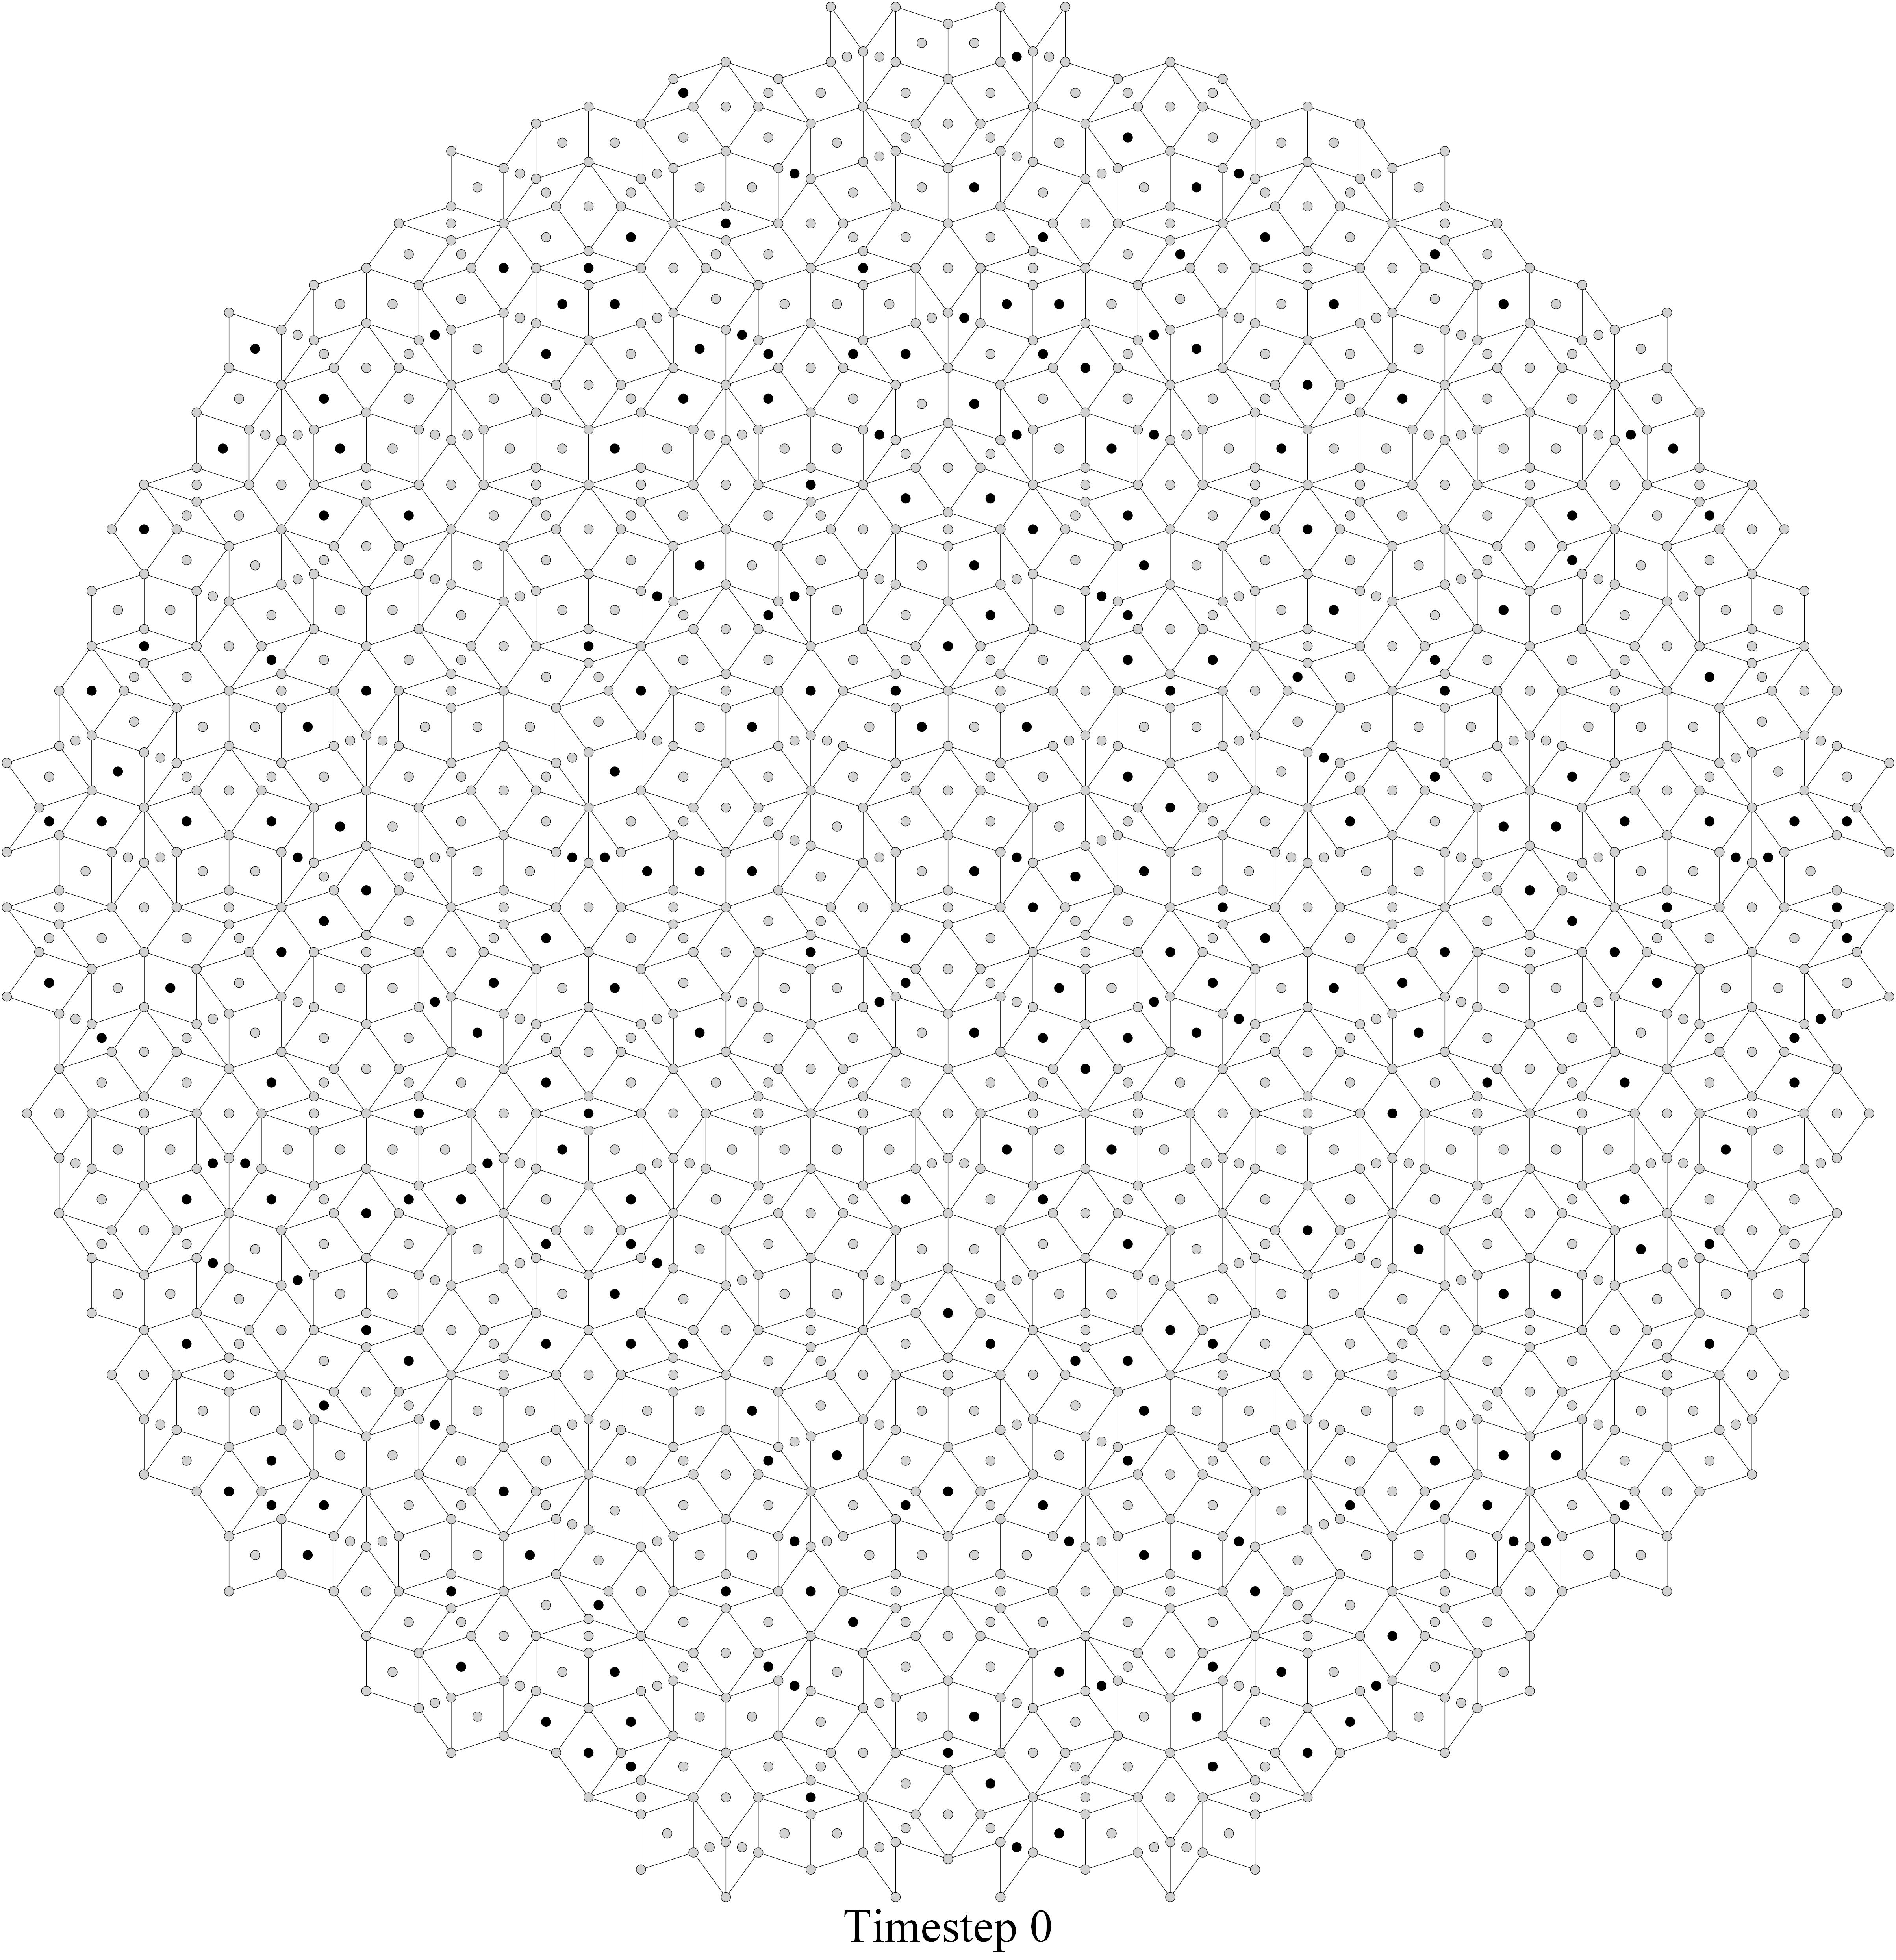
\includegraphics[width=0.2\columnwidth]{ch4_figs/crh_long/crh_long_0}}&
\subcaptionbox{}{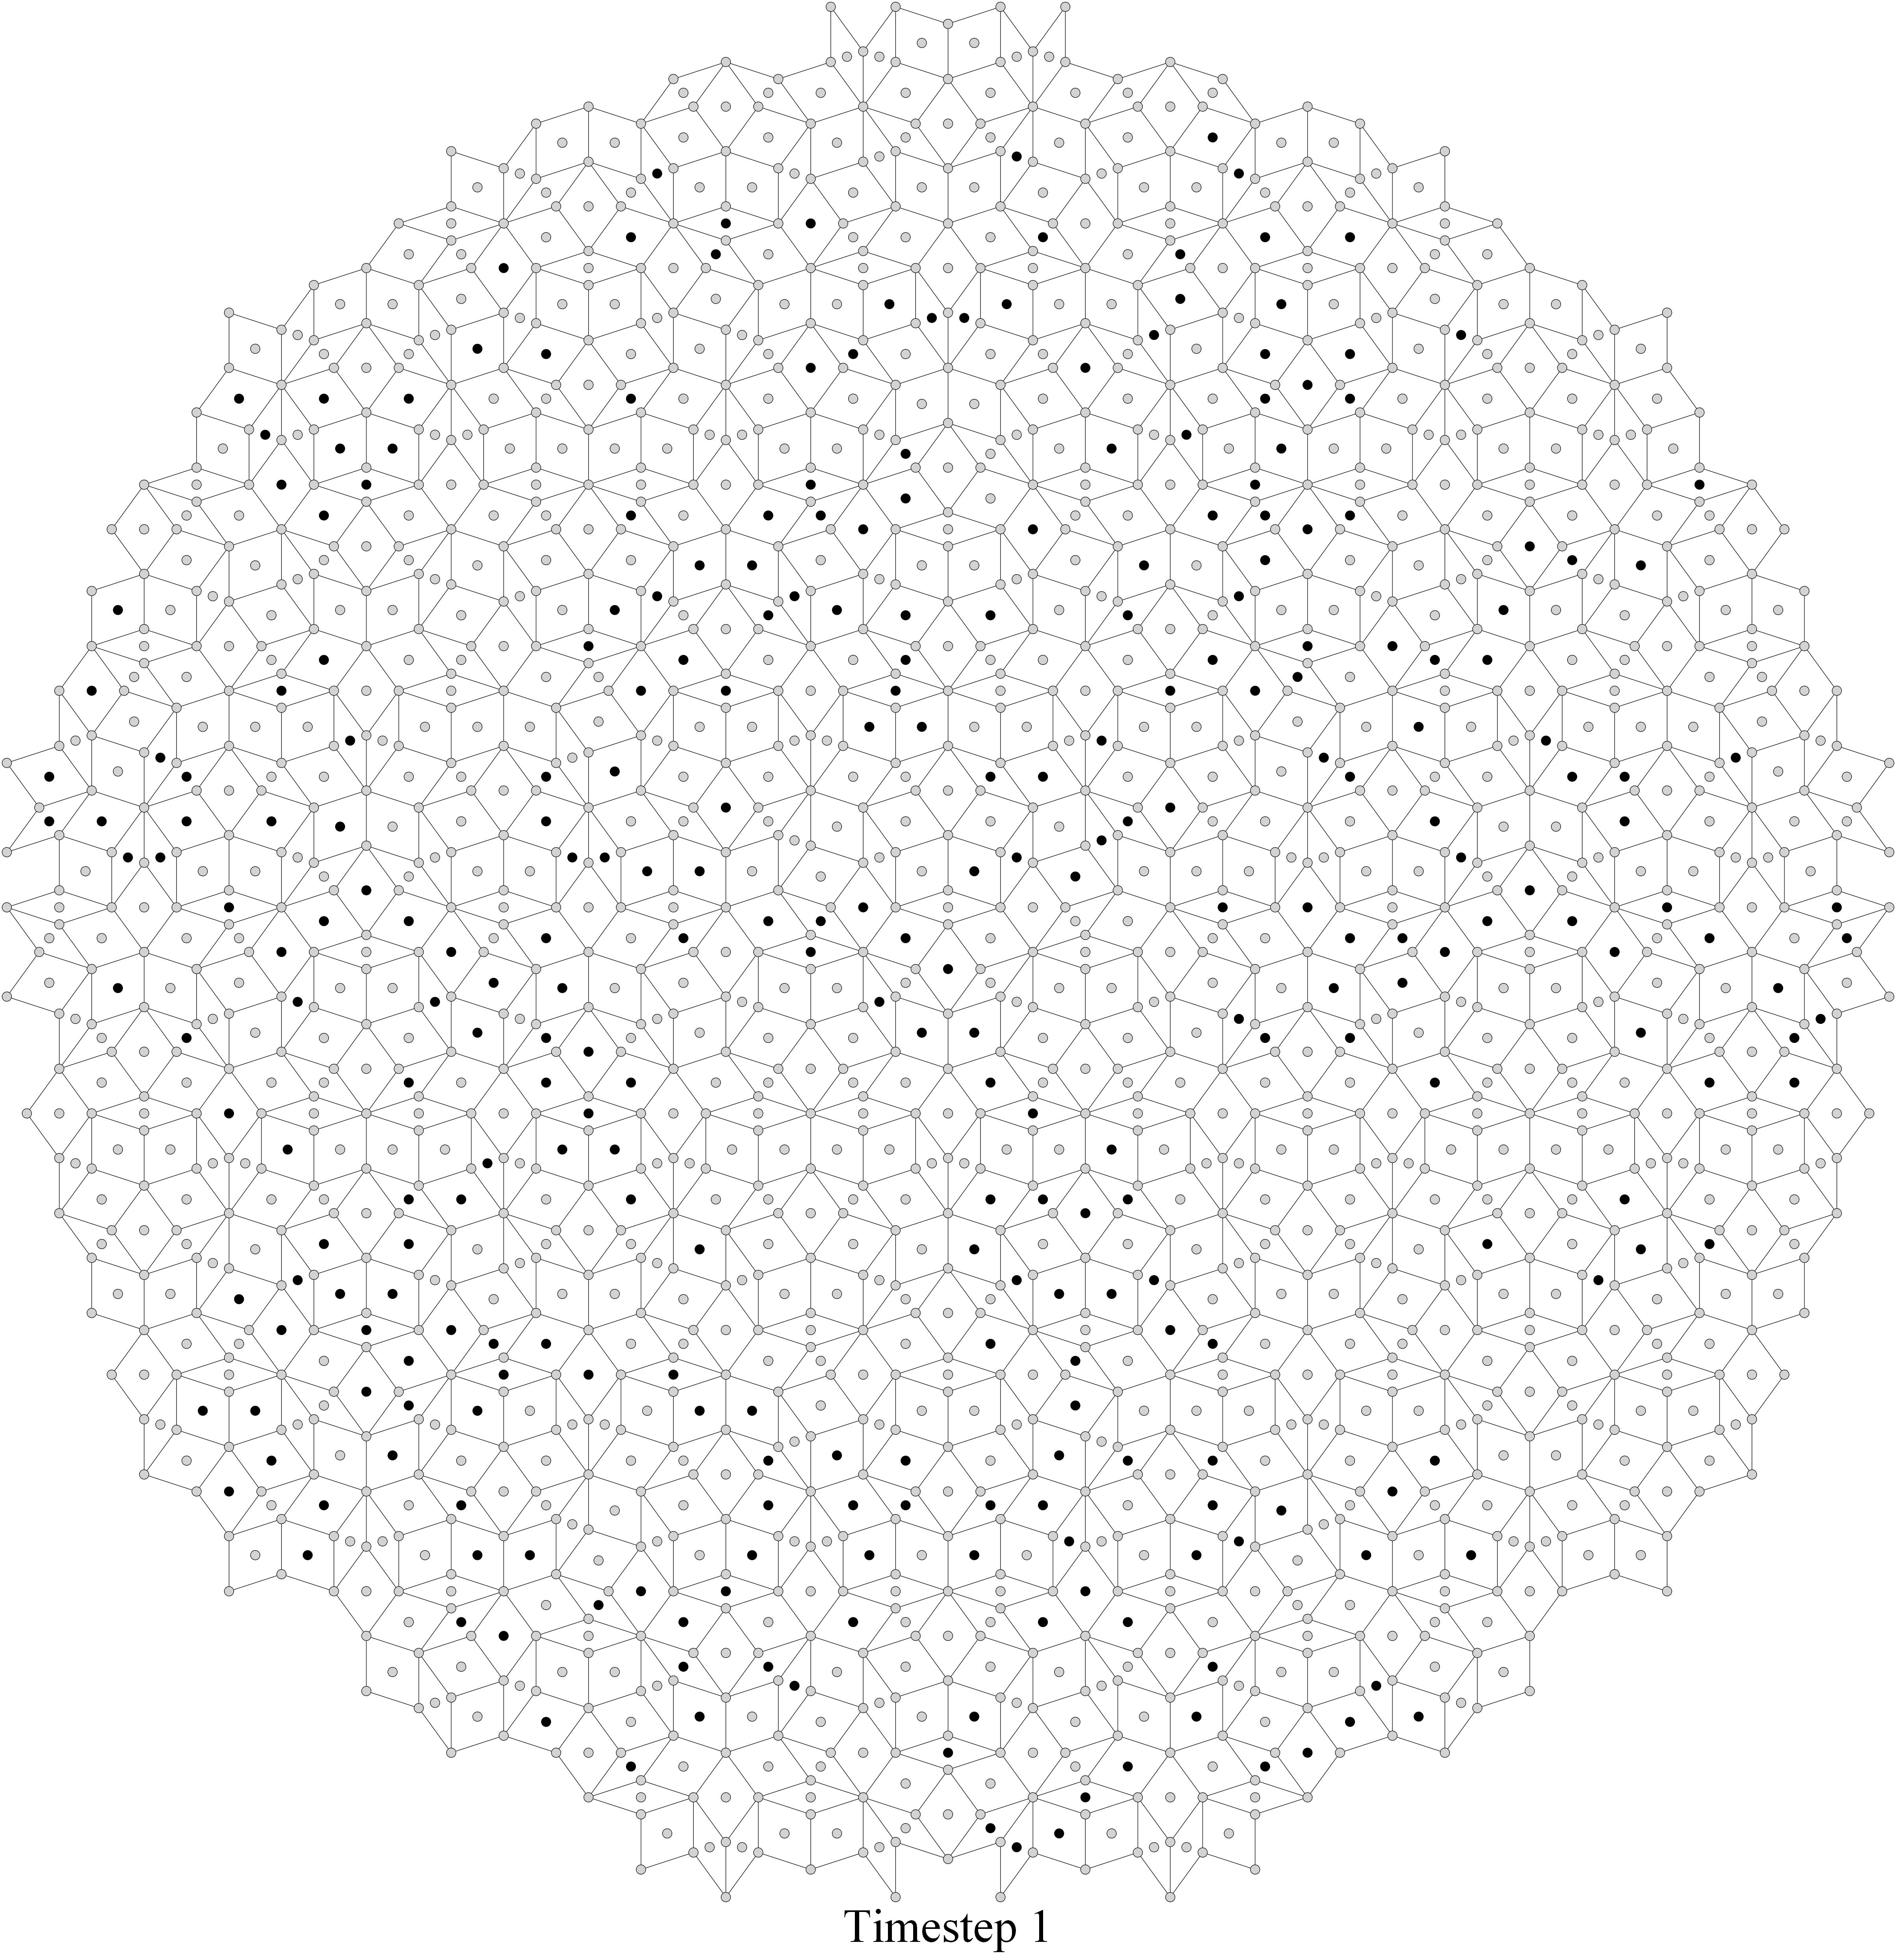
\includegraphics[width=0.2\columnwidth]{ch4_figs/crh_long/crh_long_1}}&
\subcaptionbox{}{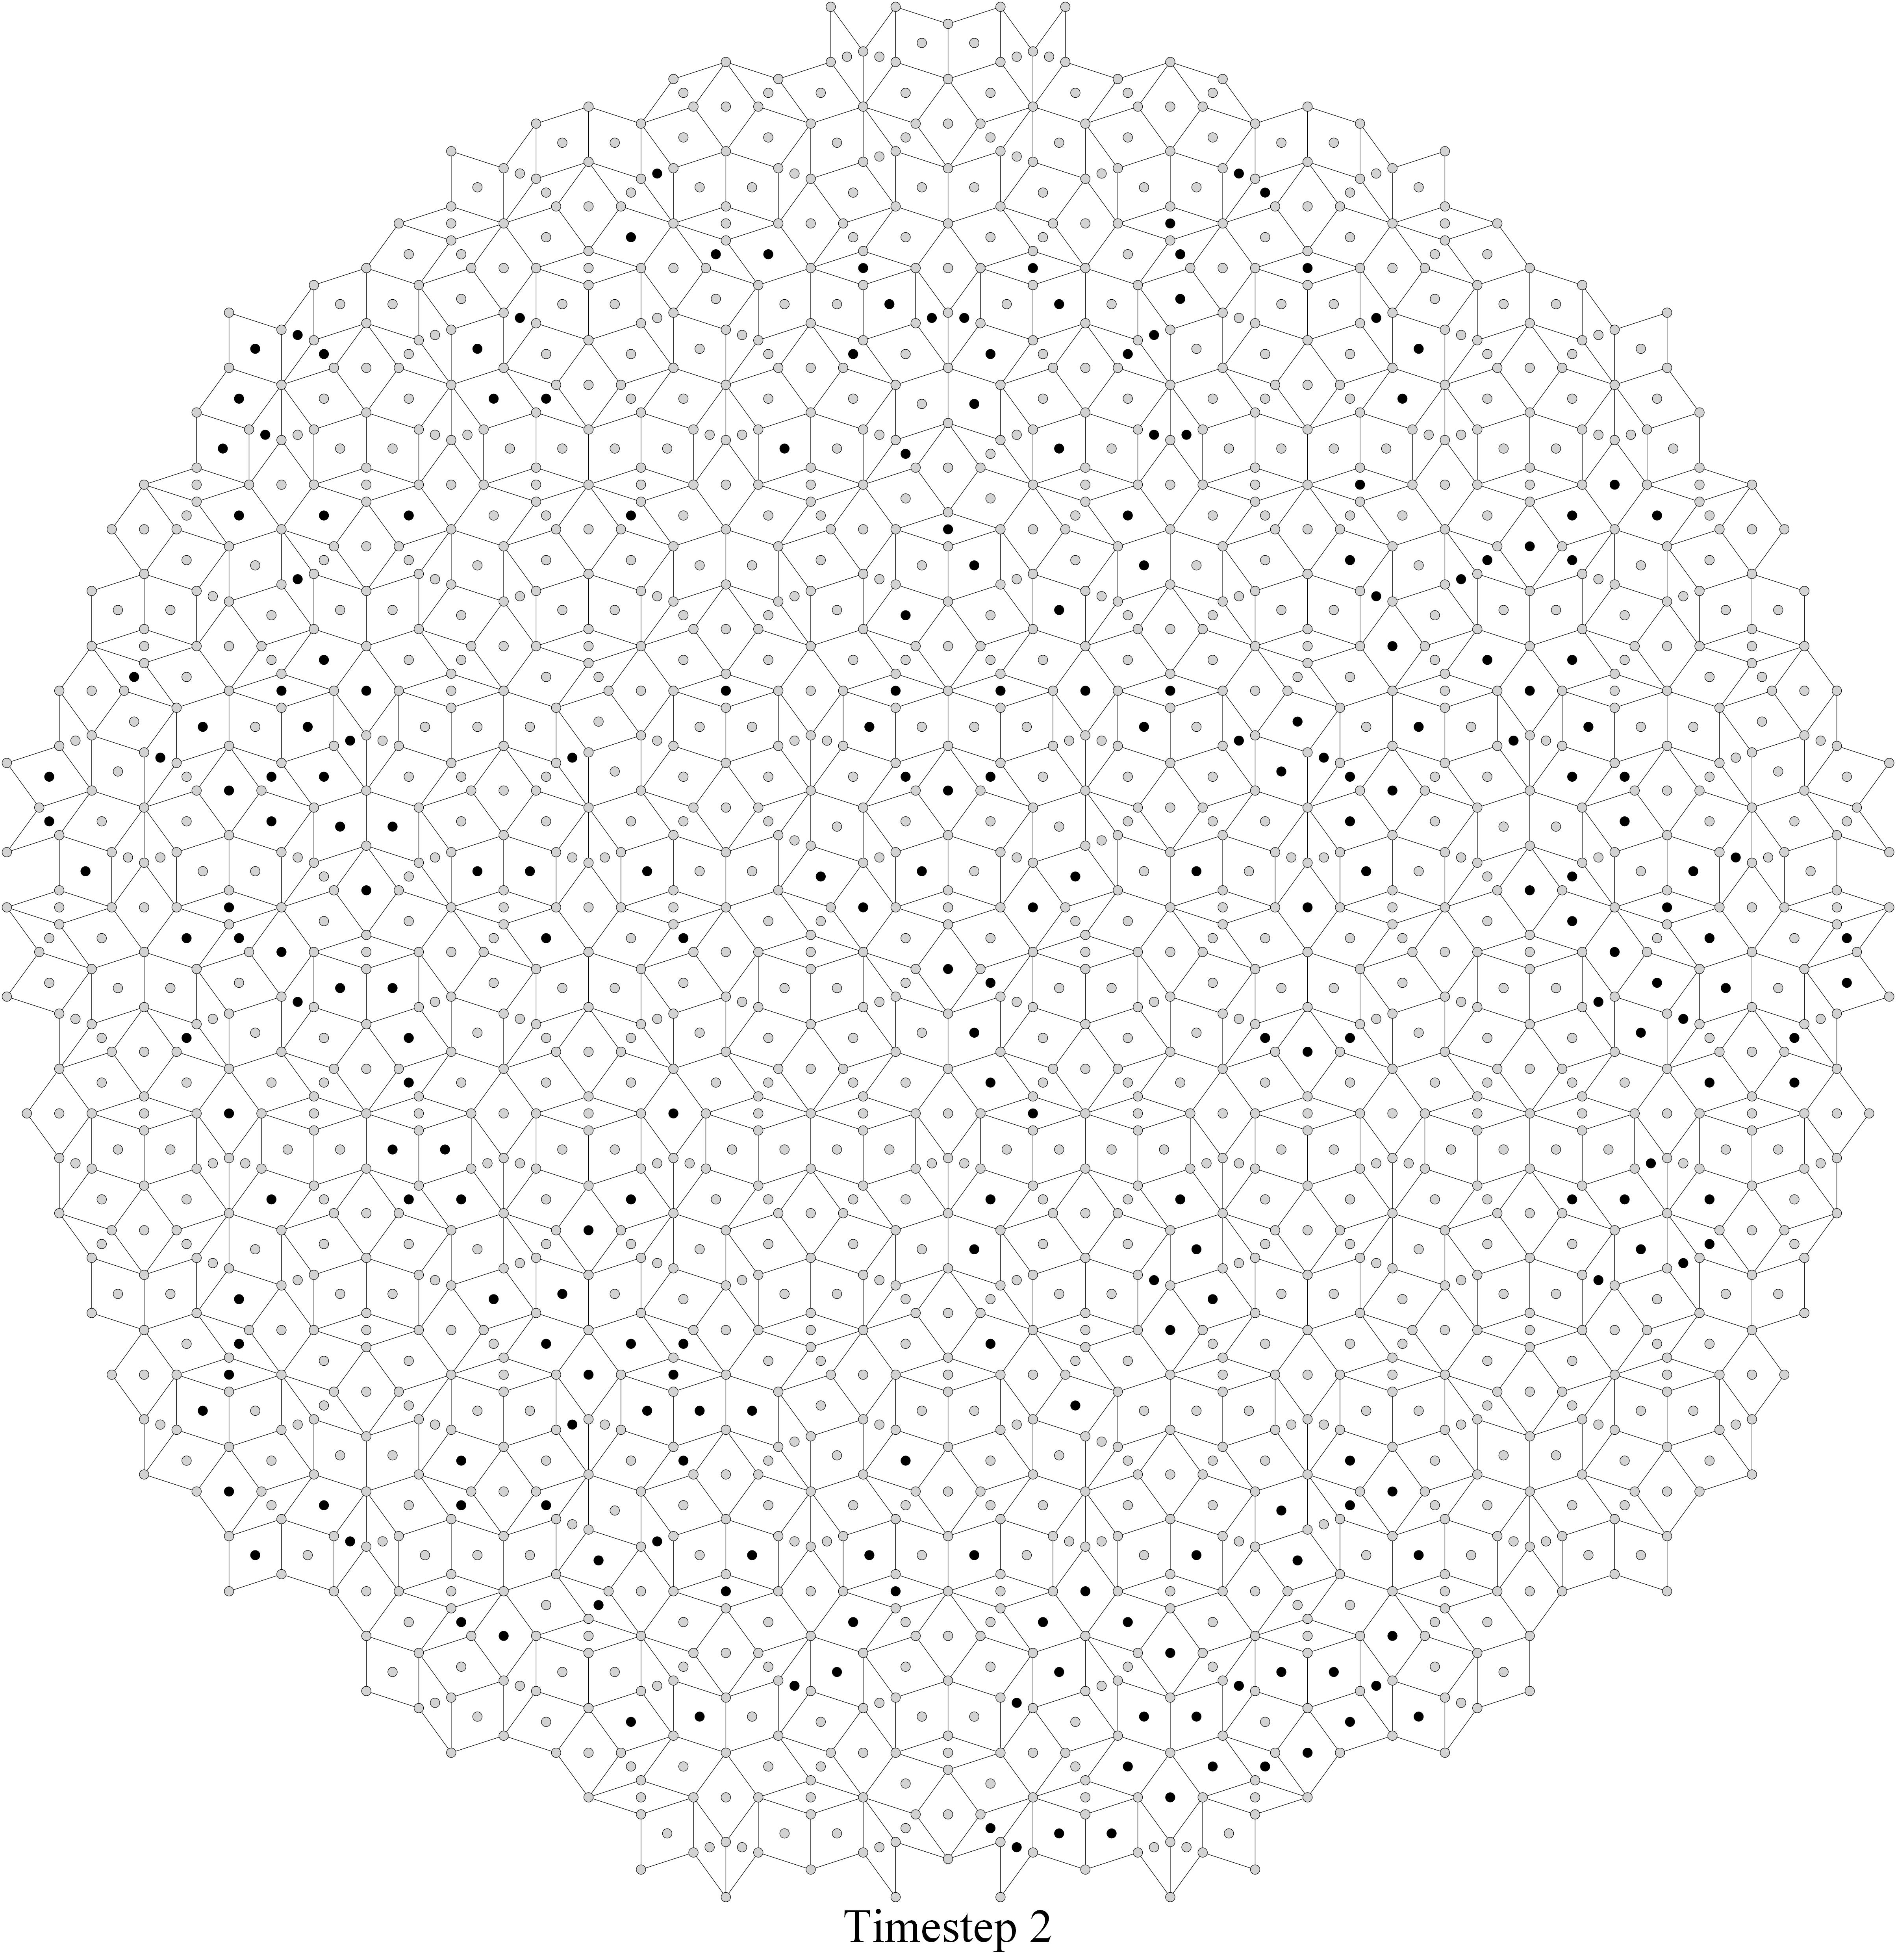
\includegraphics[width=0.2\columnwidth]{ch4_figs/crh_long/crh_long_2}}&
\subcaptionbox{}{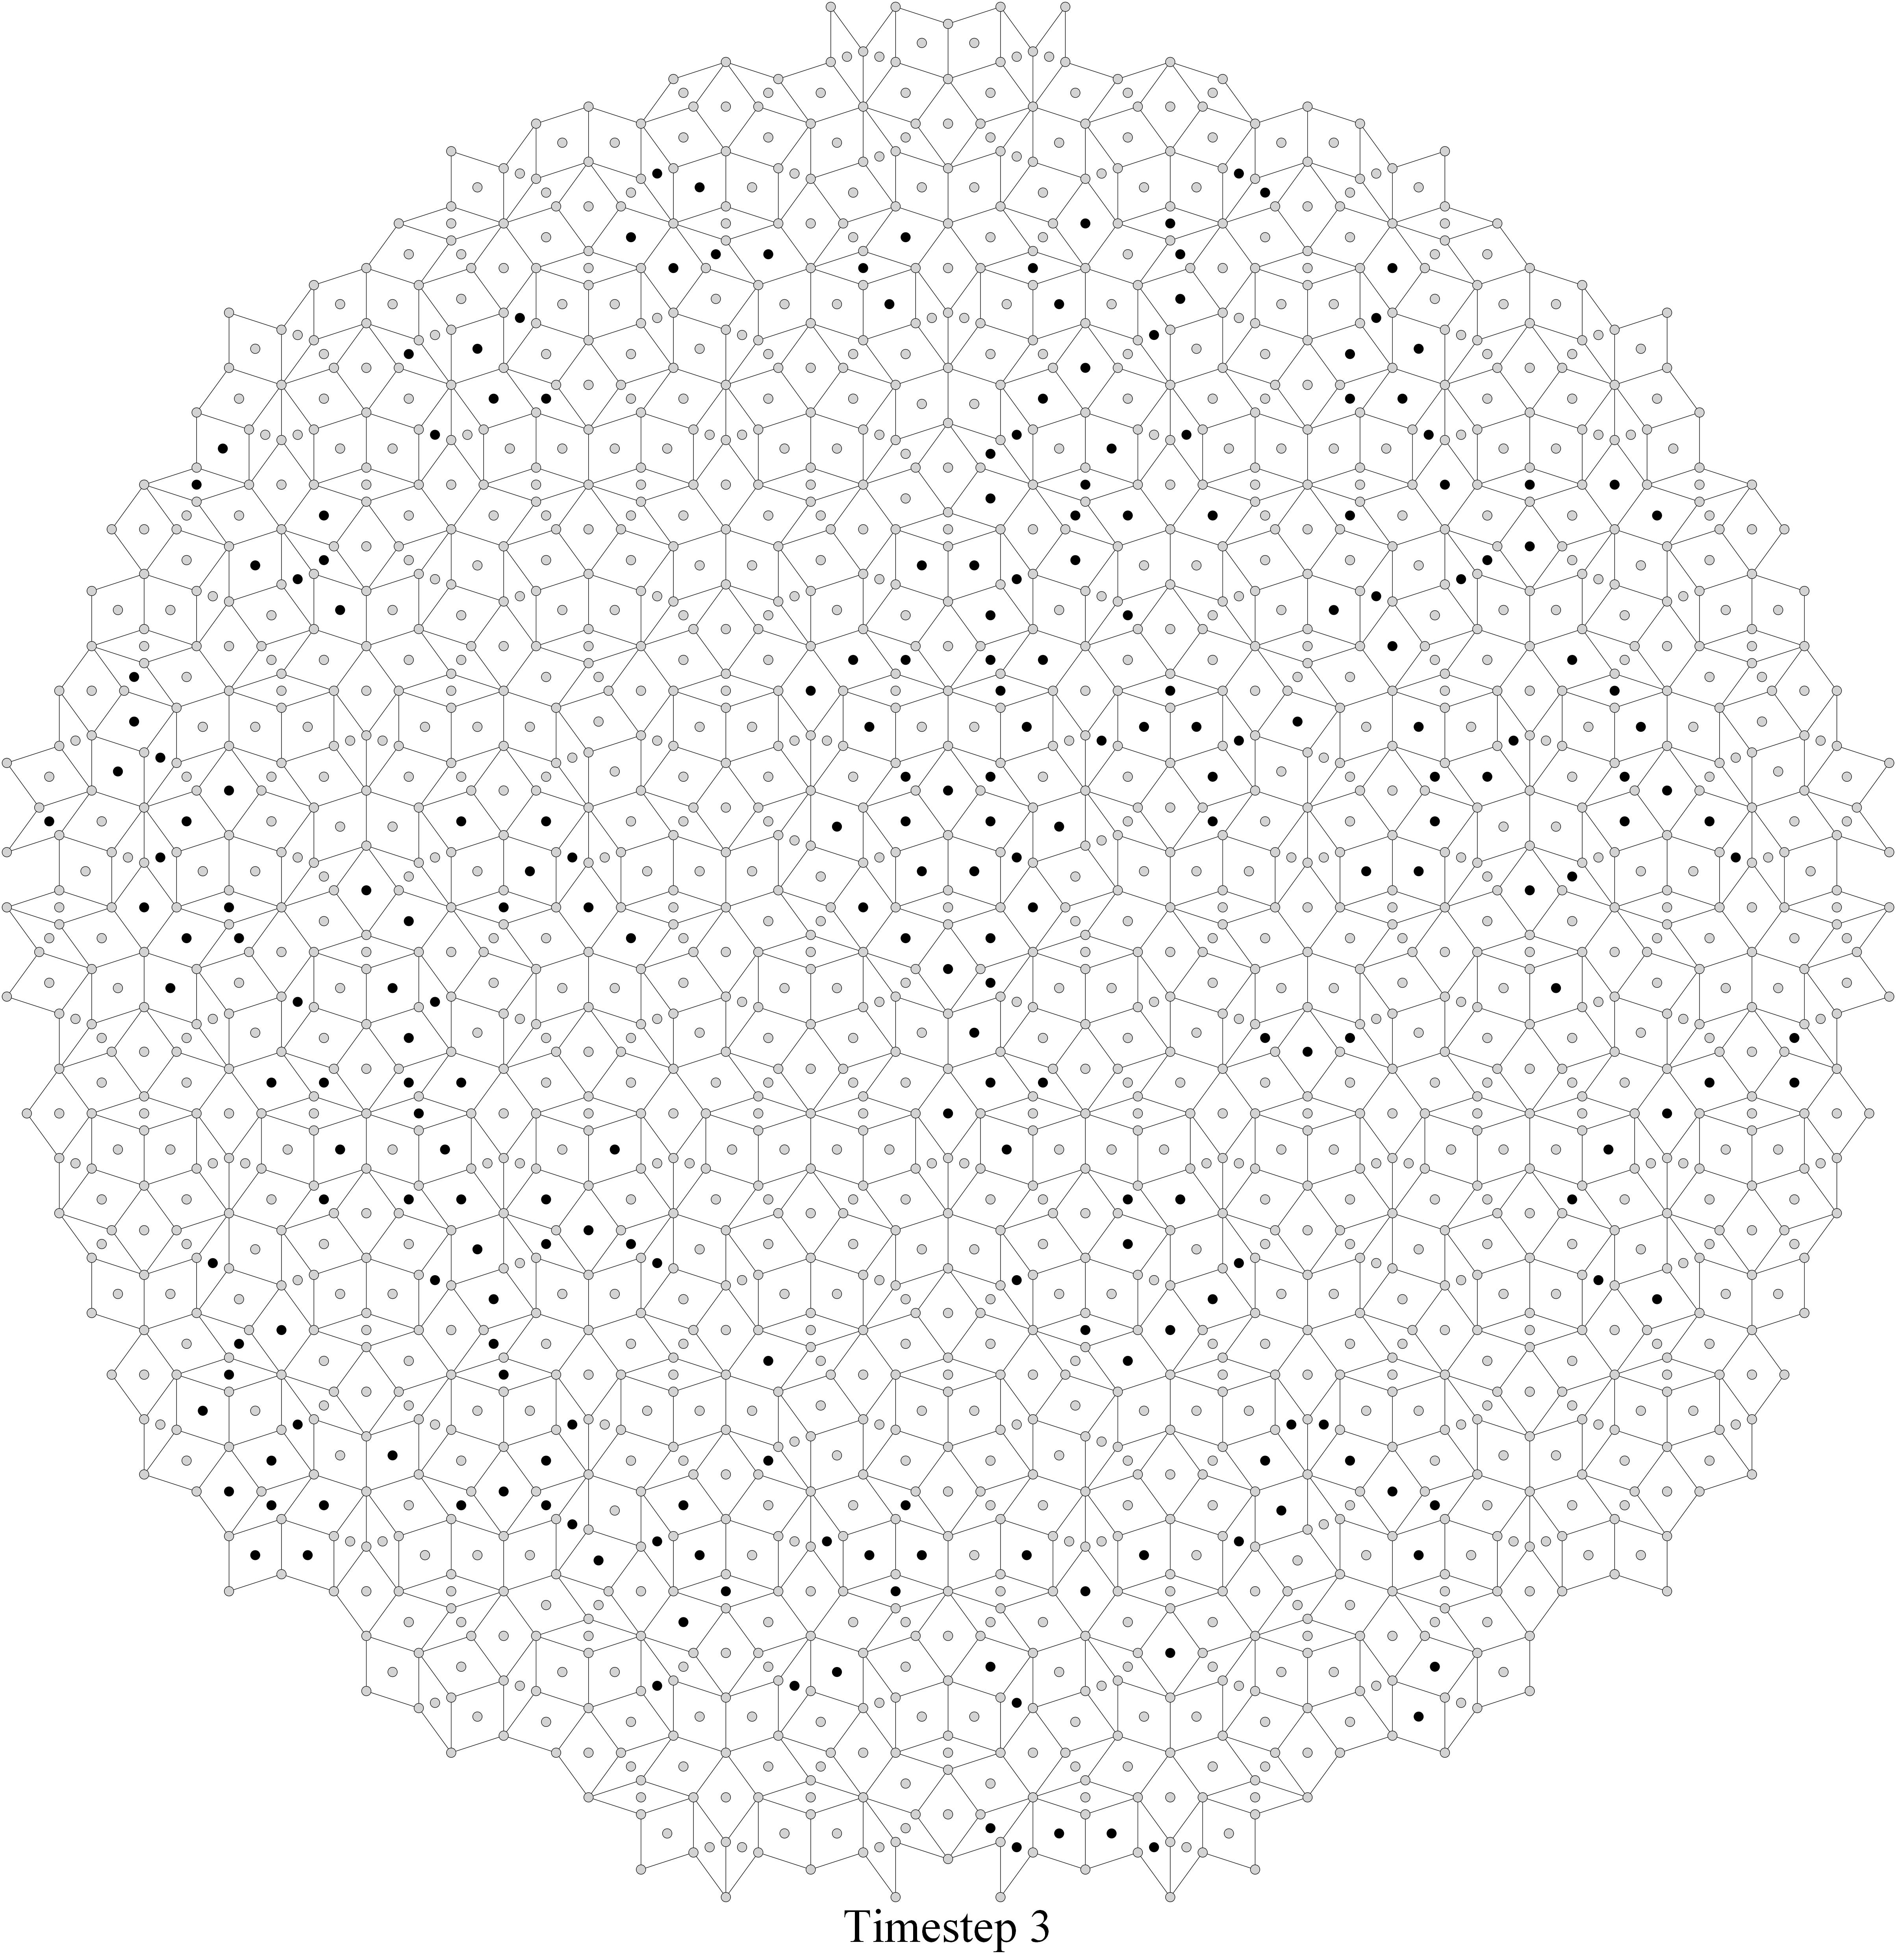
\includegraphics[width=0.2\columnwidth]{ch4_figs/crh_long/crh_long_3}}\\
}




\iffalse
\multido{\i=0+1}{66}{
    \subcaptionbox{\i}{\includegraphics[width=0.2\columnwidth]{ch4_figs/crh_long/crh_long_\i}}&
    \subcaptionbox{\i}{\includegraphics[width=0.2\columnwidth]{ch4_figs/crh_long/crh_long_\i}}&
    \subcaptionbox{\i}{\includegraphics[width=0.2\columnwidth]{ch4_figs/crh_long/crh_long_\i}}&
    \subcaptionbox{\i}{\includegraphics[width=0.2\columnwidth]{ch4_figs/crh_long/crh_long_\i}}\\
}
\fi

\iffalse
\begin{python}

for i in range(0,5):

    print("\subcaptionbox{}{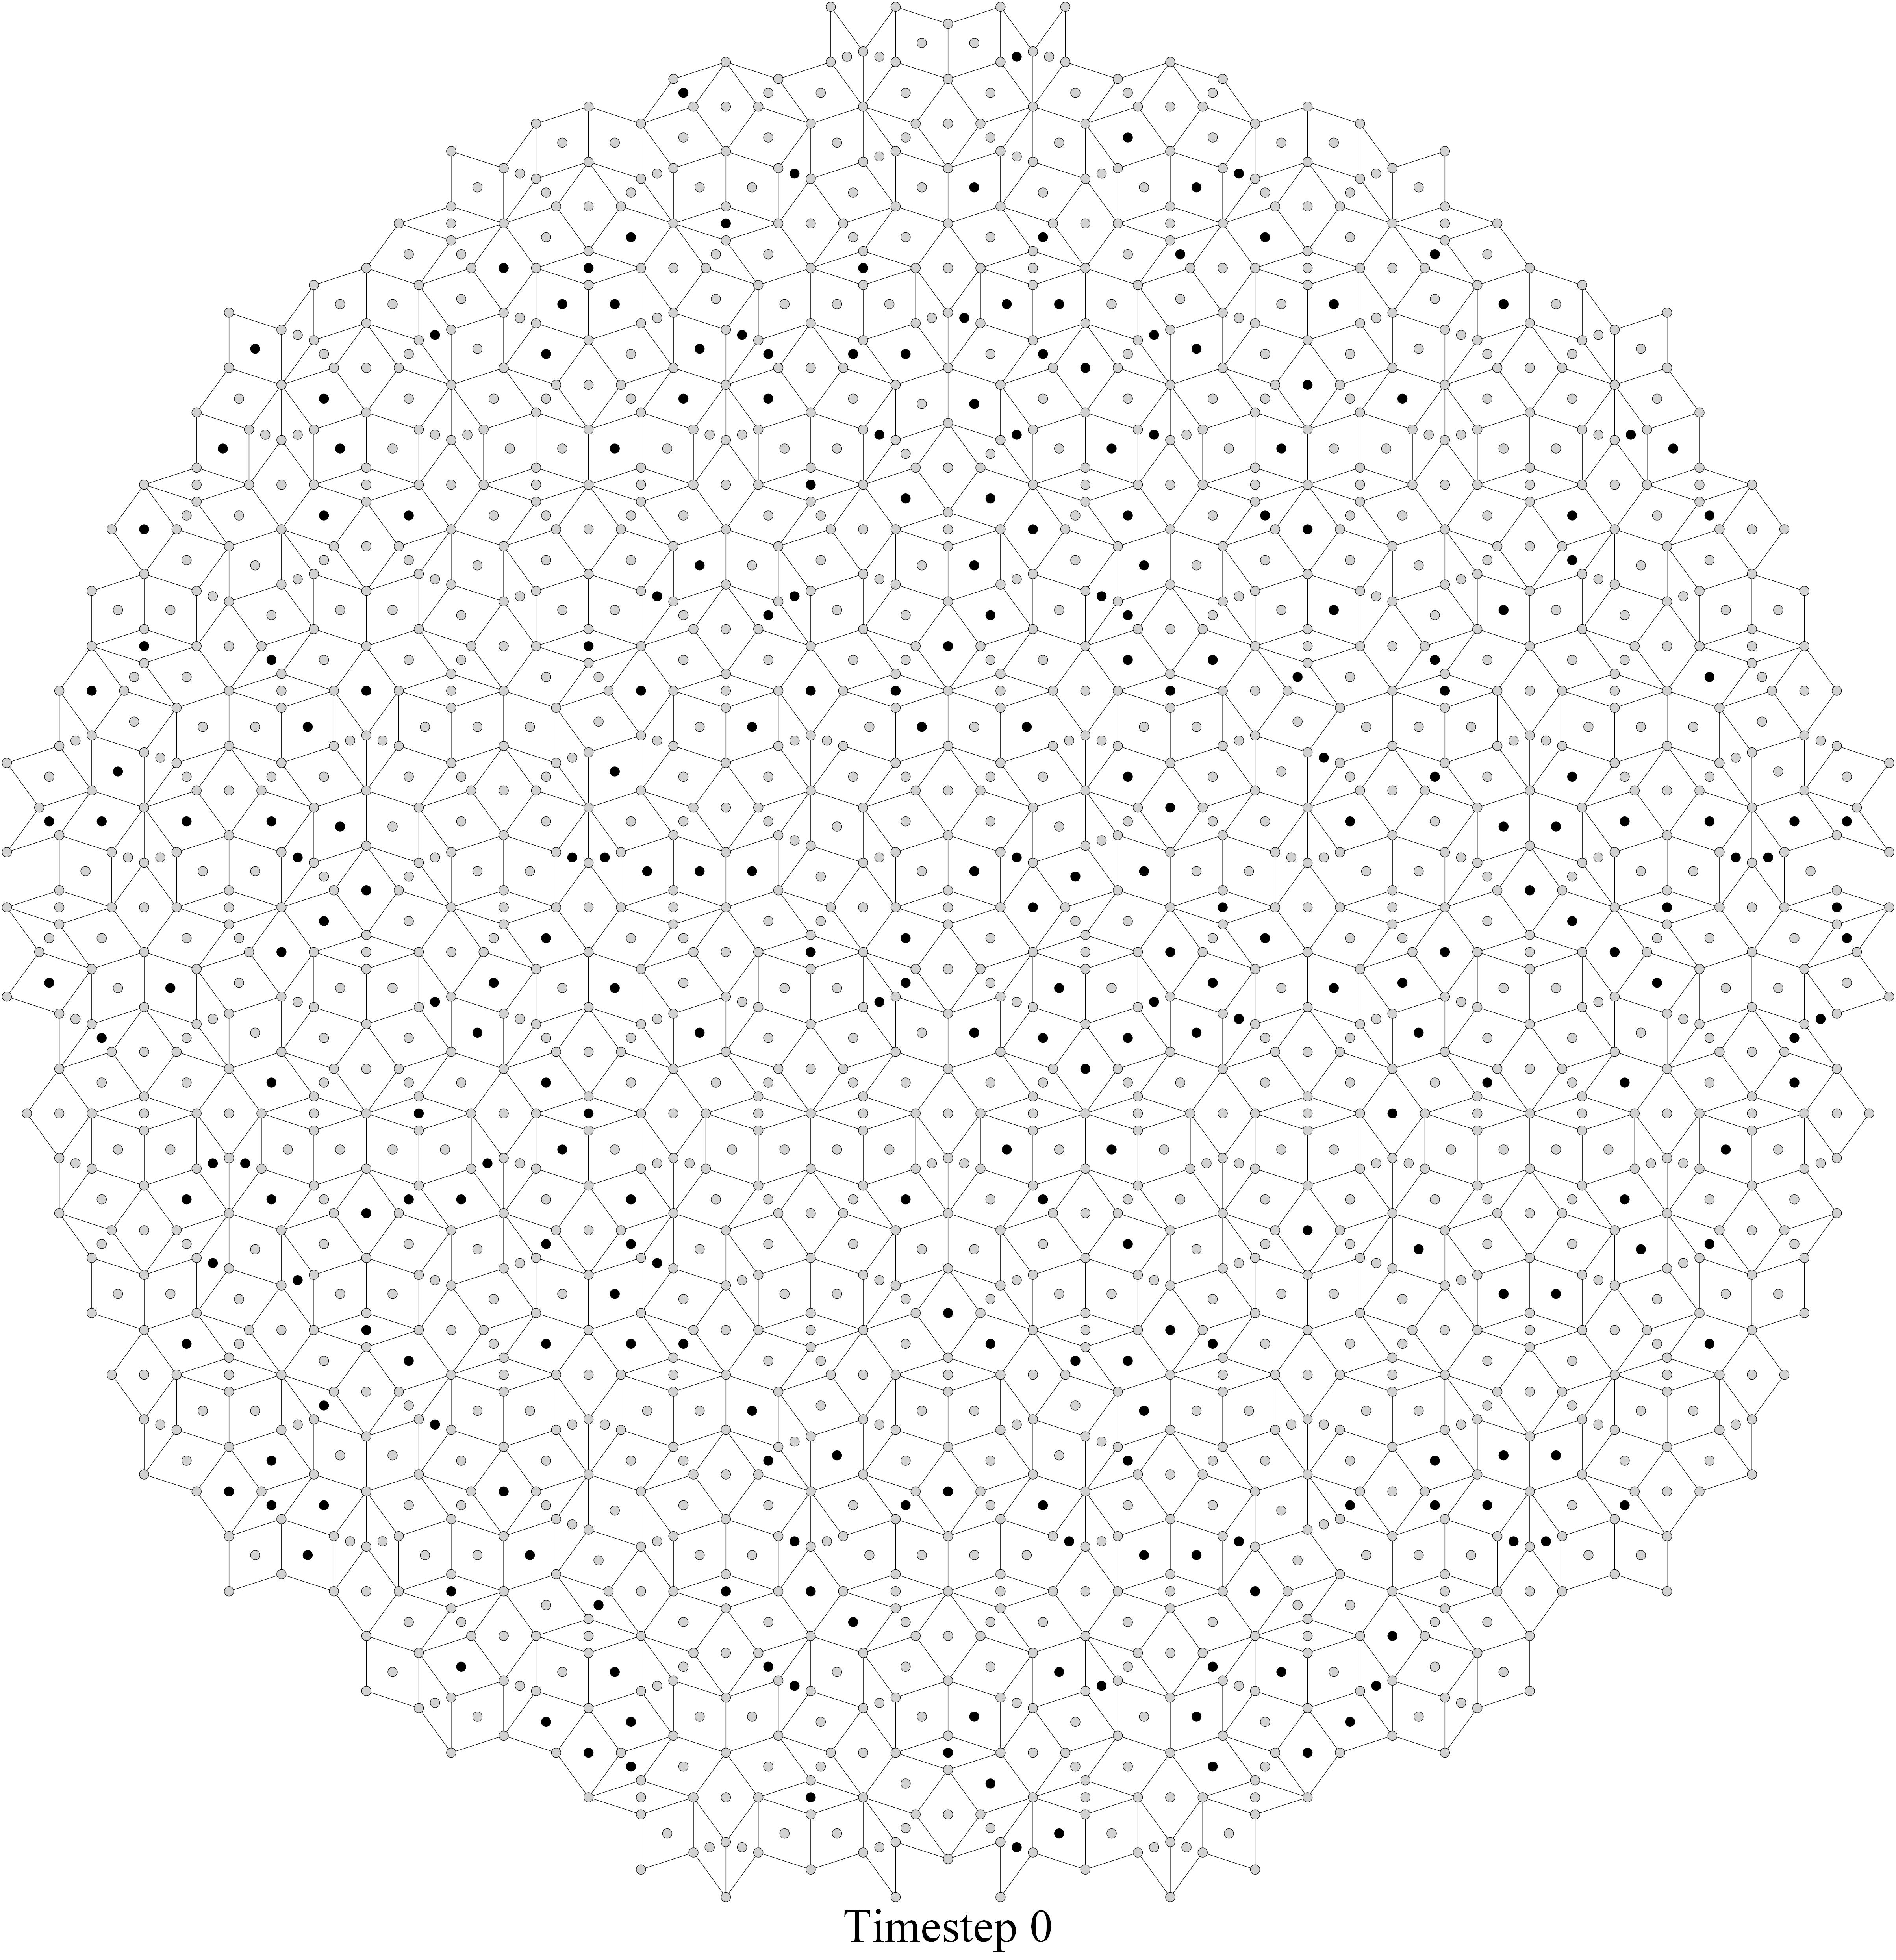
\includegraphics[width=0.2\columnwidth]{ch4_figs/crh_long/crh_long_0}}&")
    print("\subcaptionbox{}{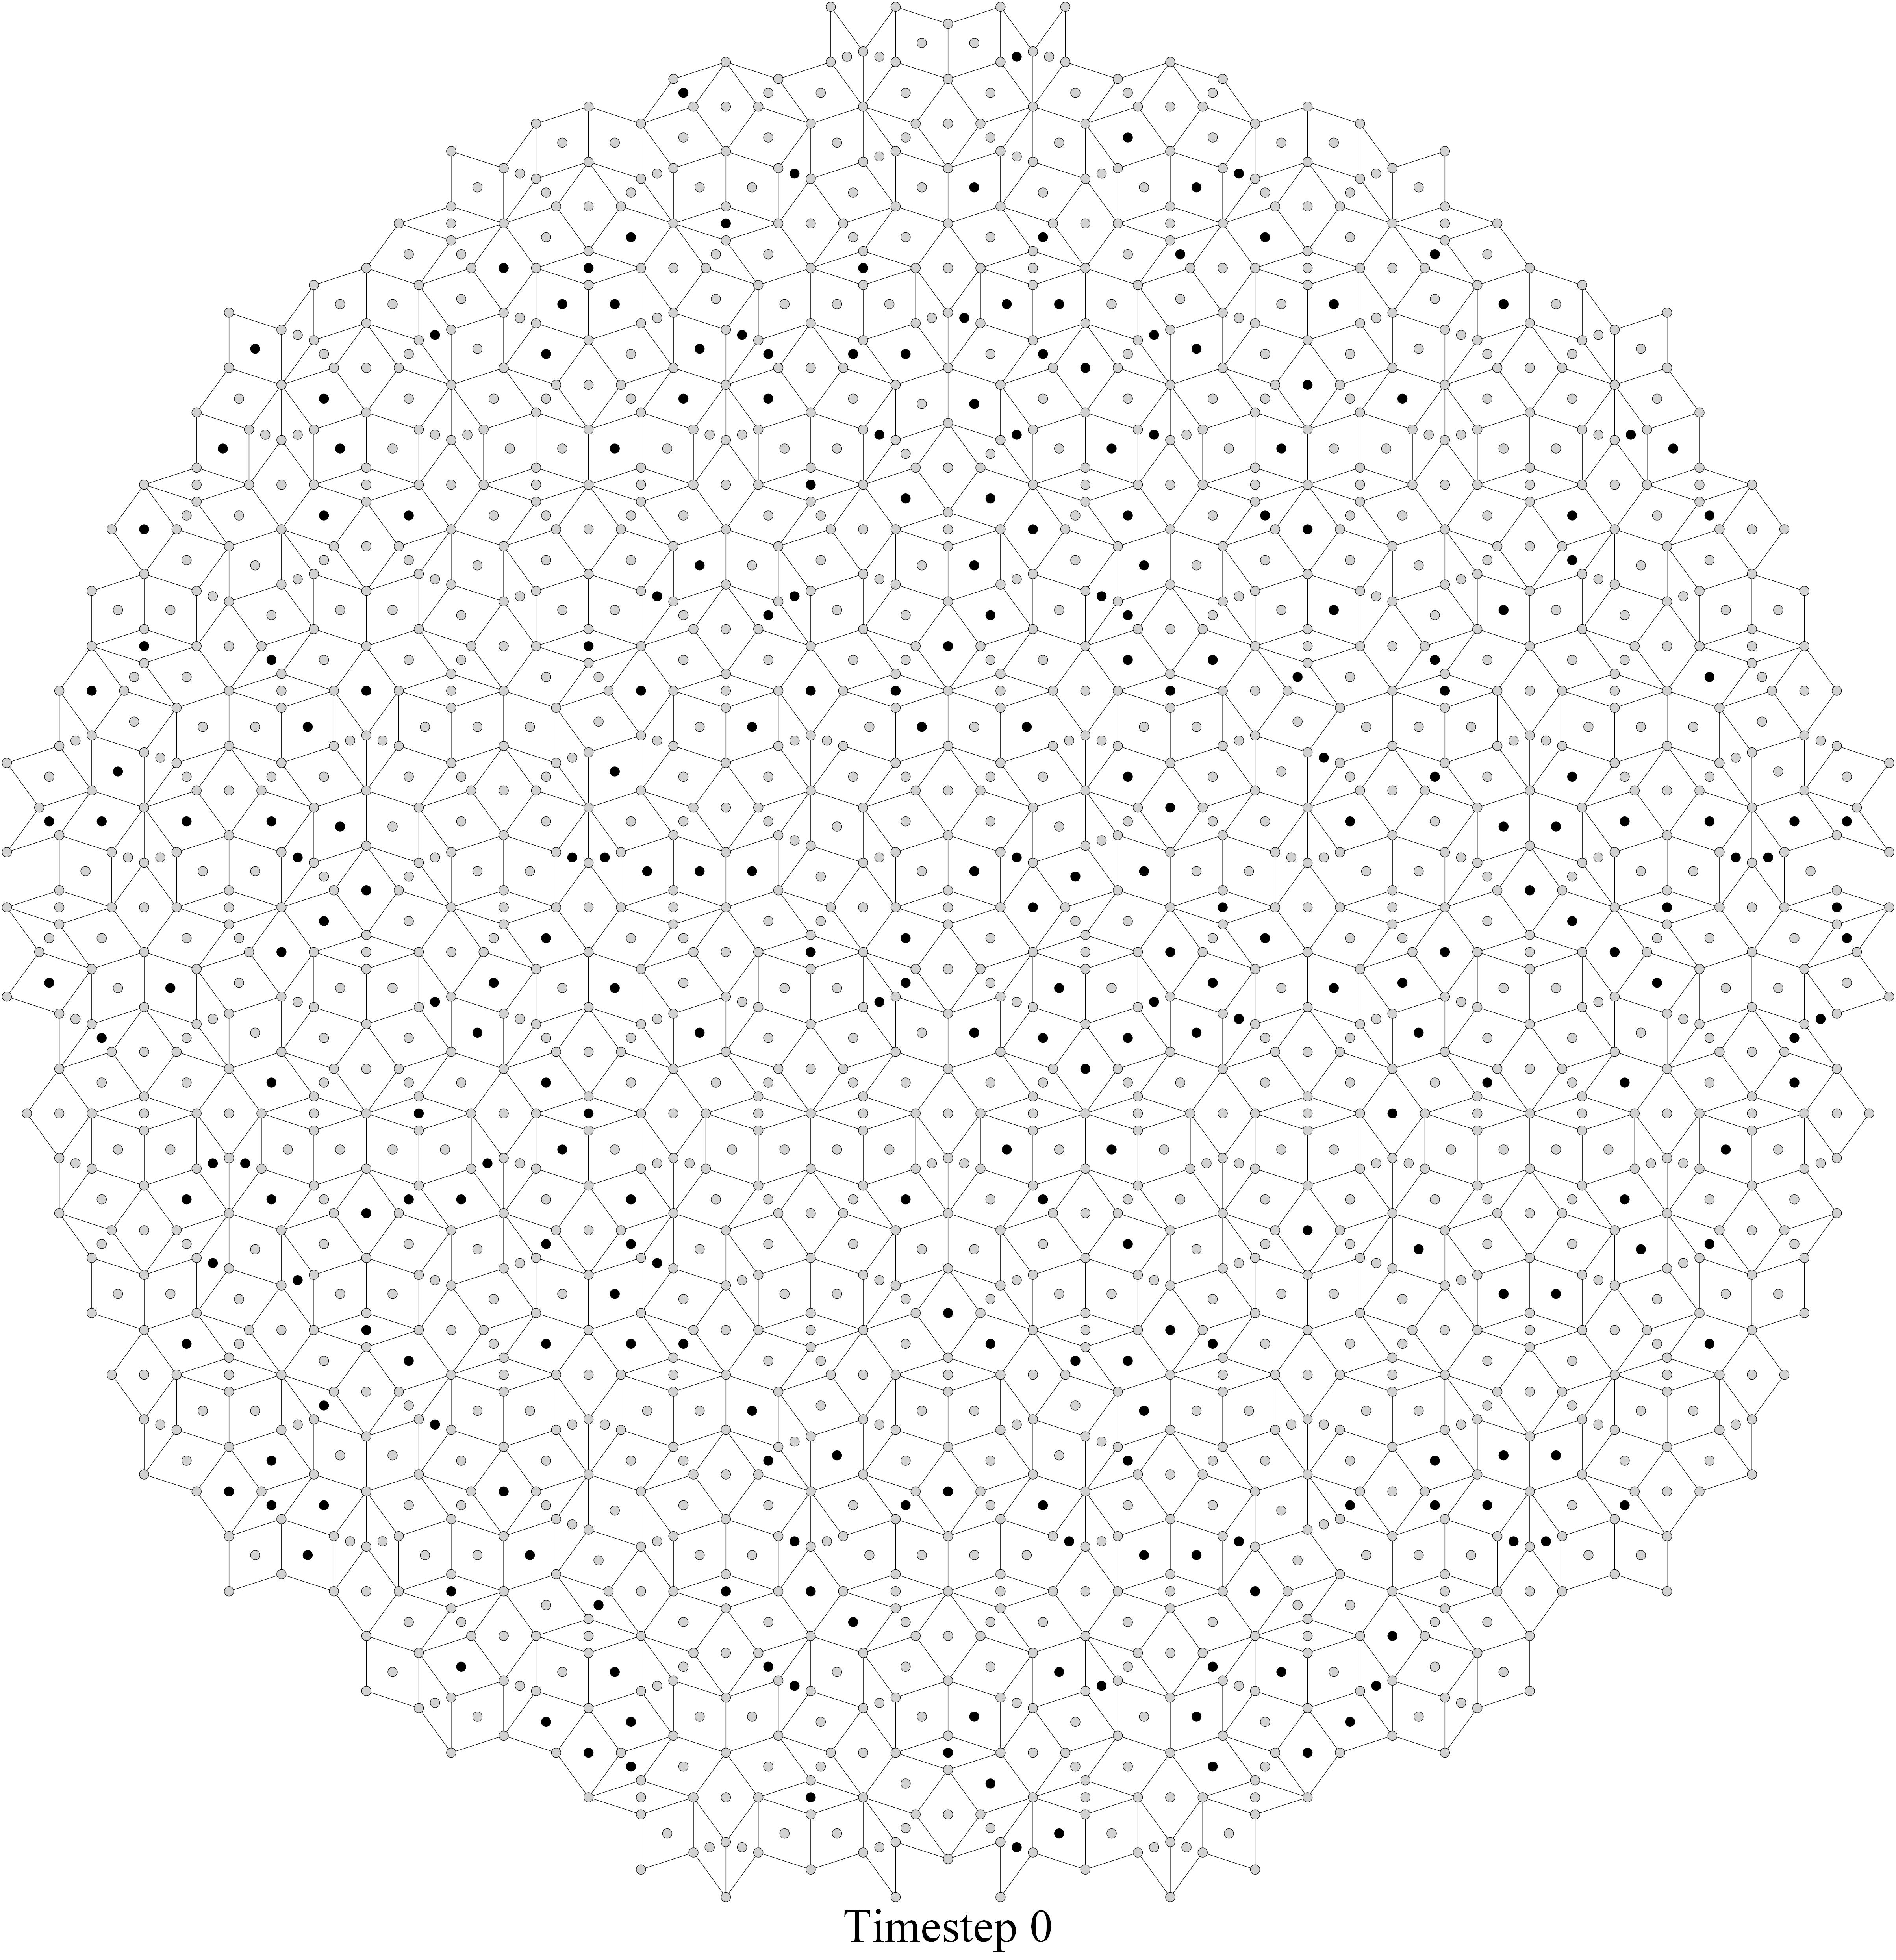
\includegraphics[width=0.2\columnwidth]{ch4_figs/crh_long/crh_long_0}}&")   
    print("\subcaptionbox{}{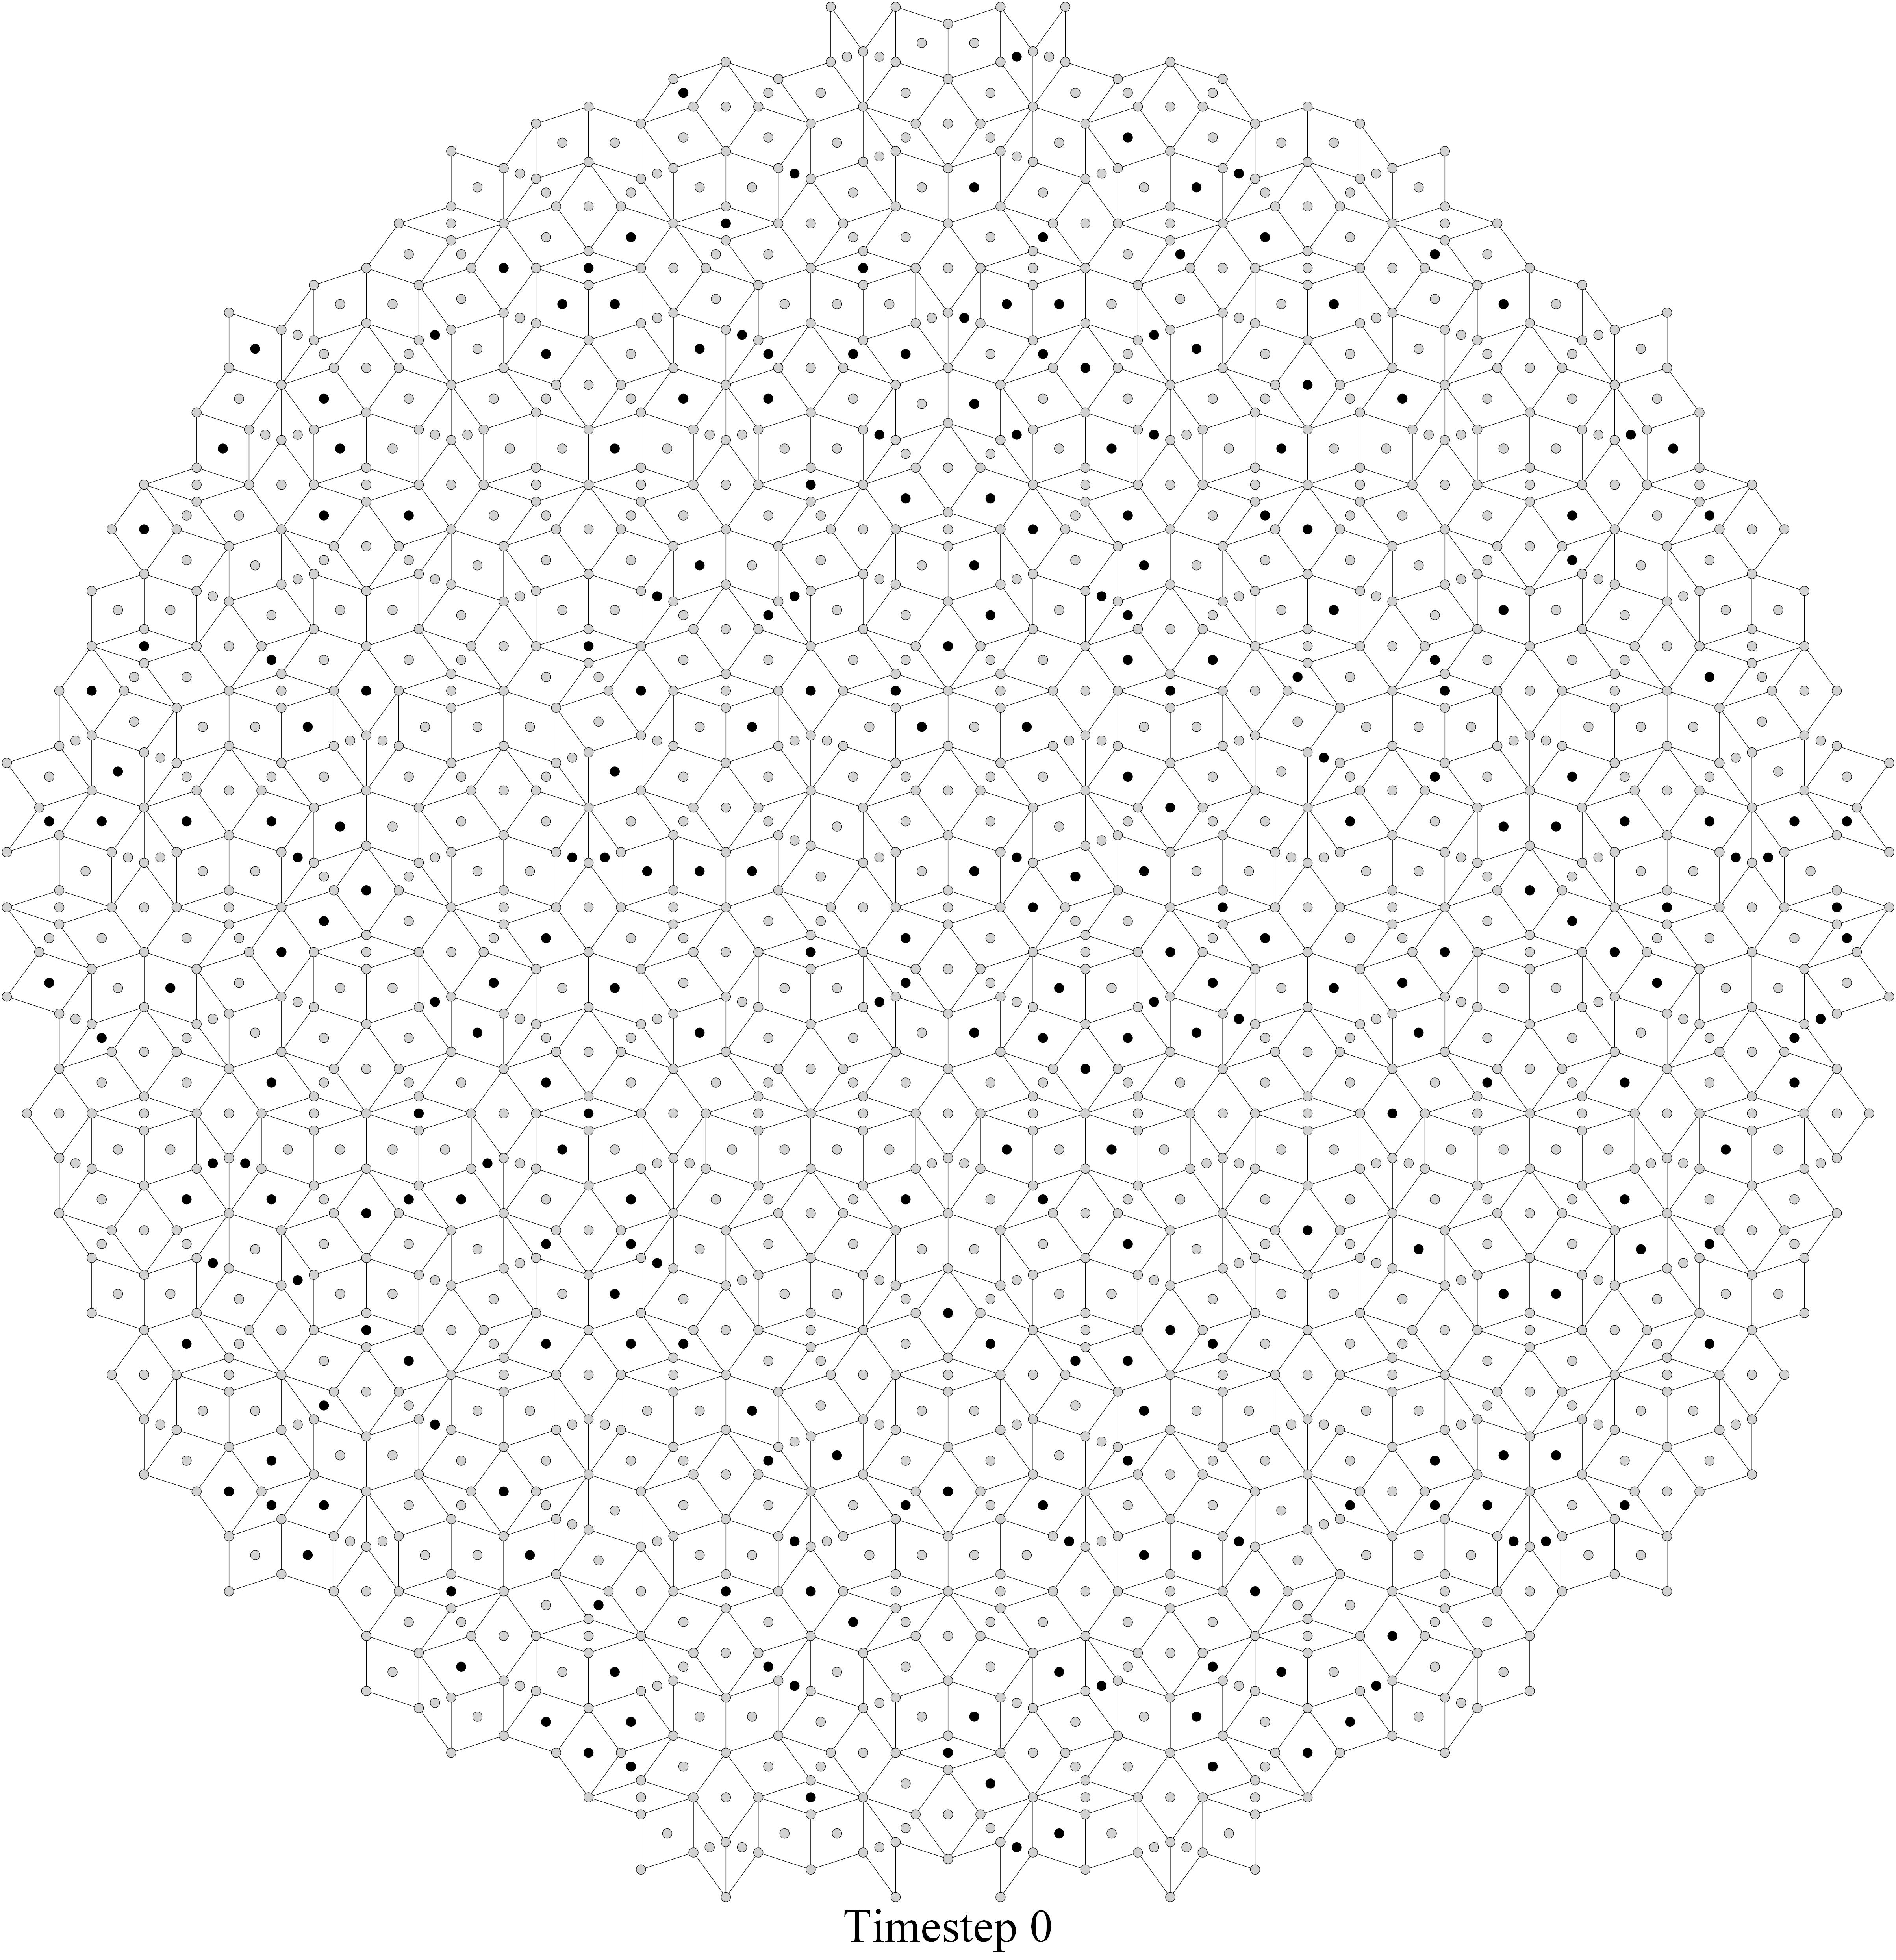
\includegraphics[width=0.2\columnwidth]{ch4_figs/crh_long/crh_long_0}}&")
    print("\subcaptionbox{}{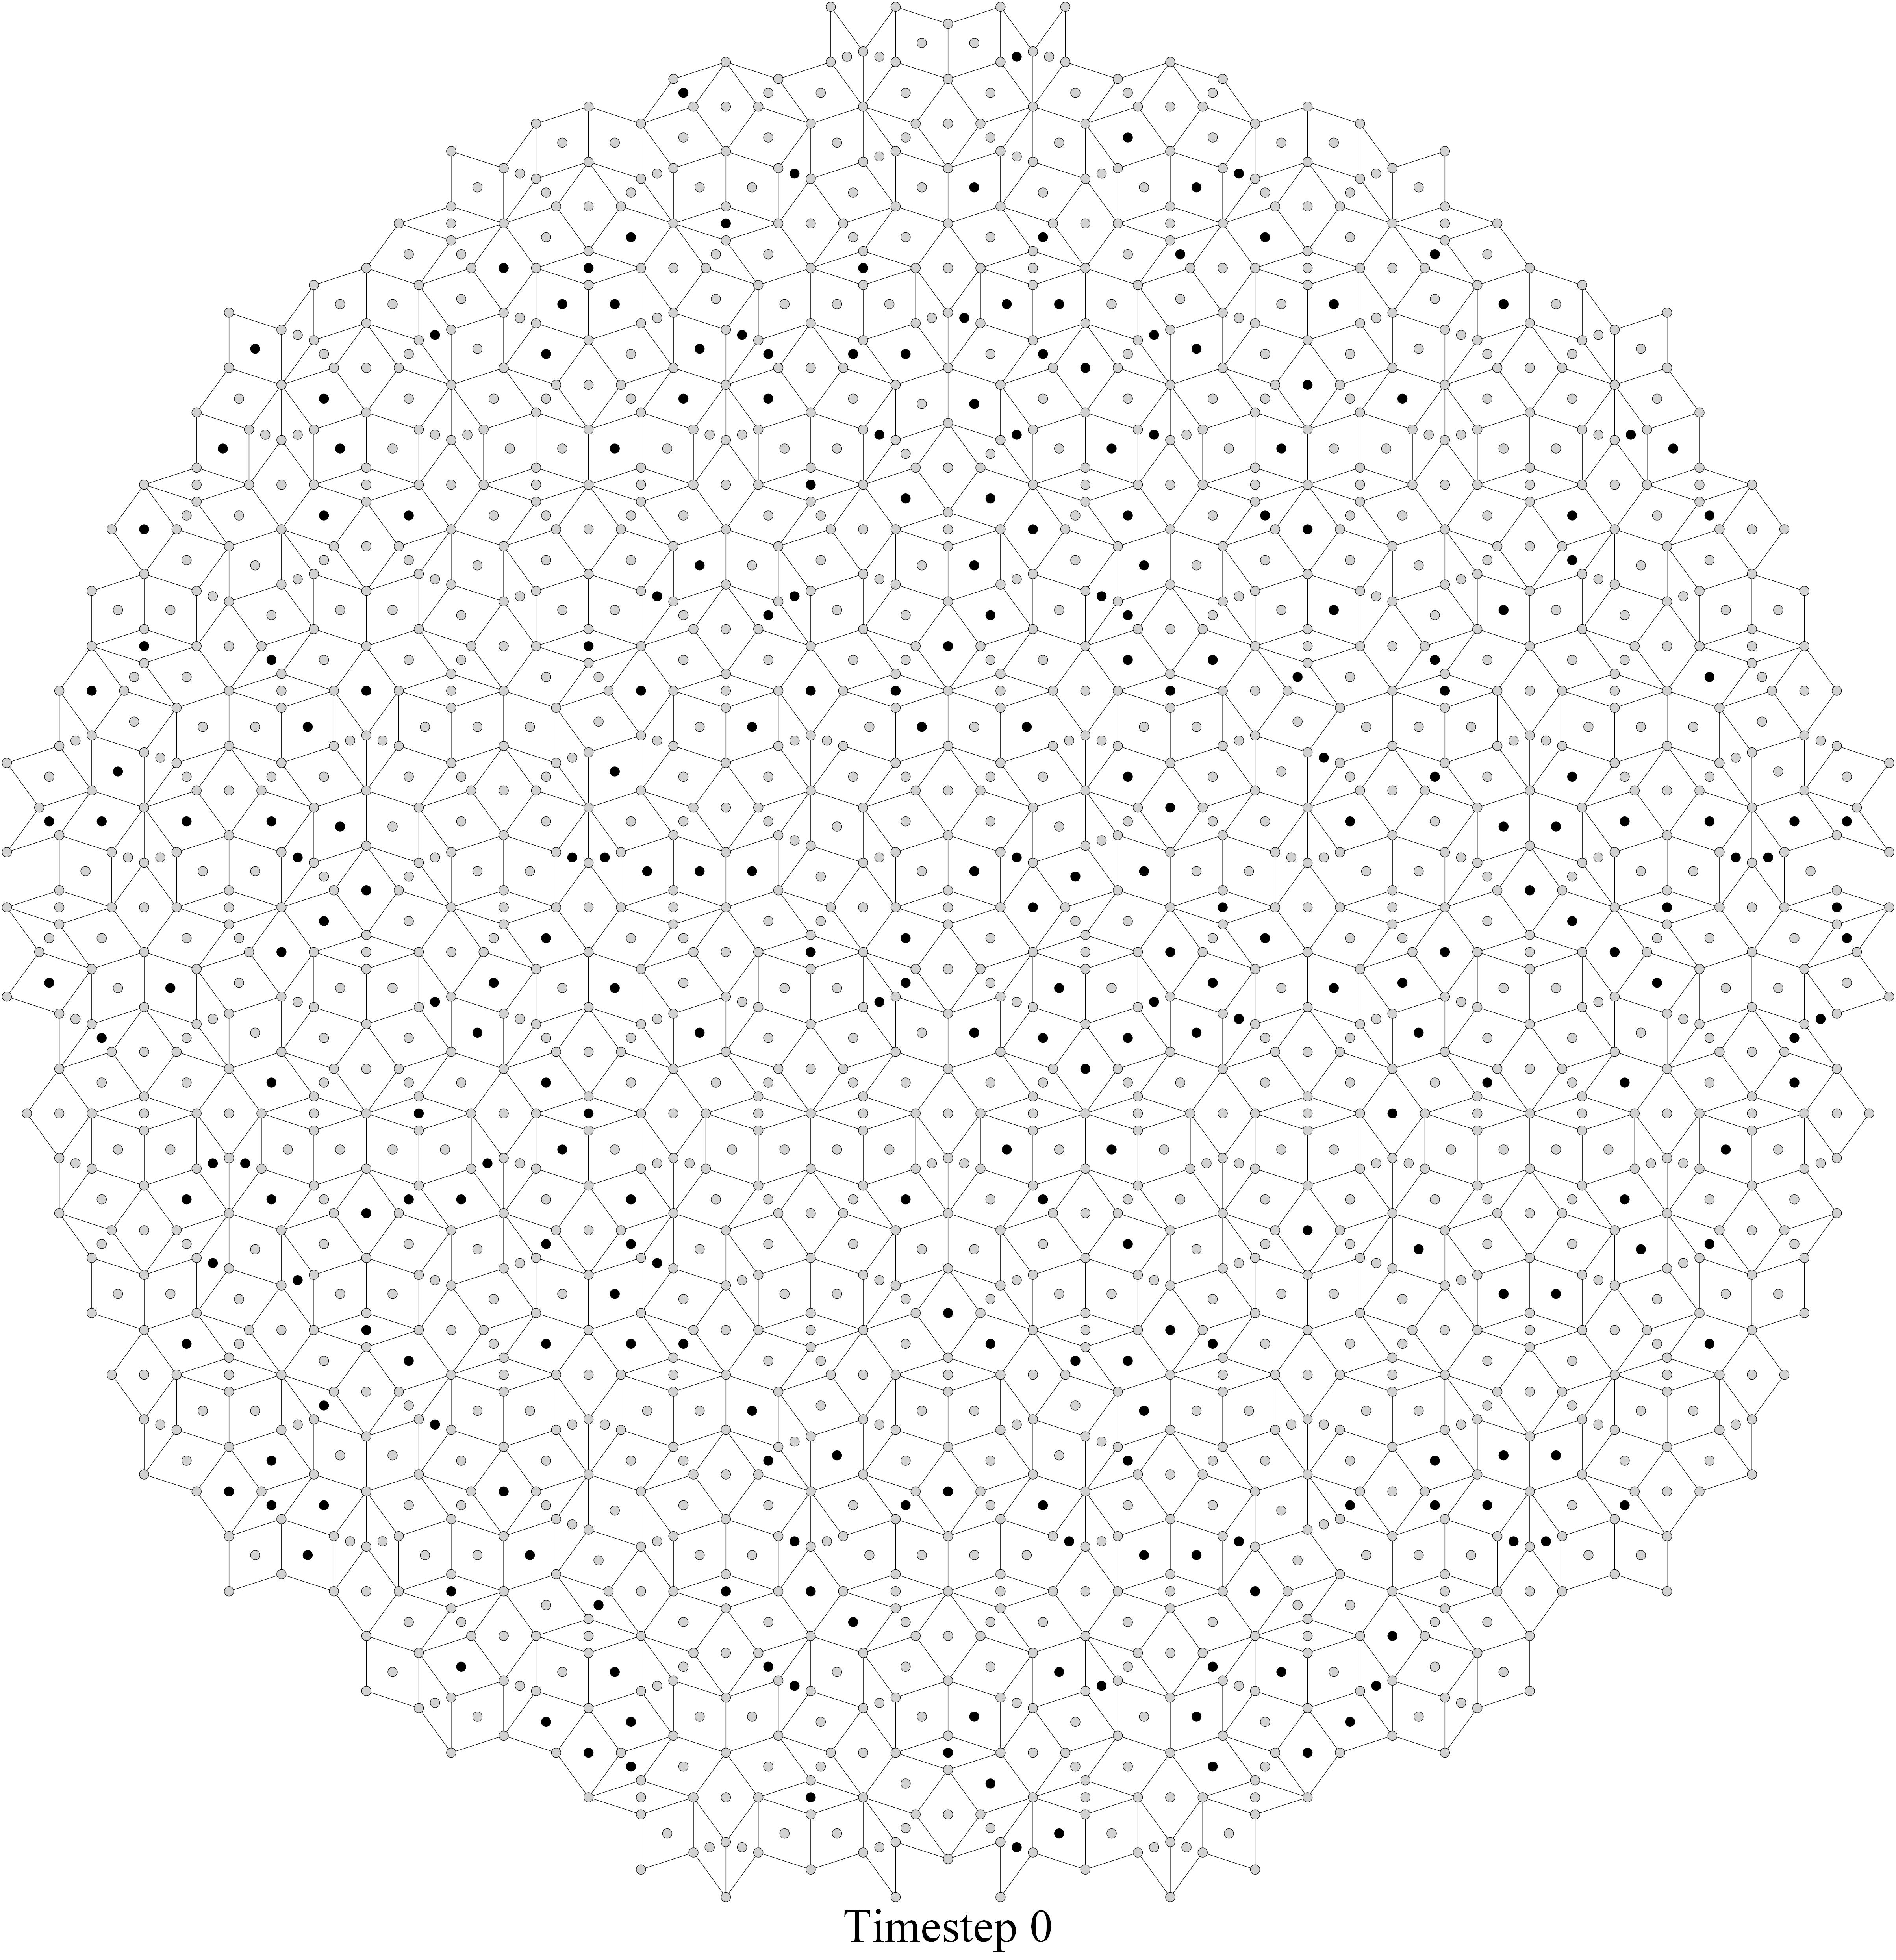
\includegraphics[width=0.2\columnwidth]{ch4_figs/crh_long/crh_long_0}}\\")
\end{python}


\makeatletter
\newwrite\Code@out

\newcommand\python{\obeylines\expandafter\pythonArg\noexpand}

\newcommand\pythonArg[1][tmp.py.in]{%
    \gdef\FNameIn{#1}
    \gdef\FNameOut{tmp.py.out}
    \begingroup
        \@bsphack%
        \immediate\openout\Code@out\FNameIn%
        \let\do\@makeother\dospecials%
        \catcode`\^^M\active%
        \def\verbatim@processline{%
            \immediate\write\Code@out{\the\verbatim@line}}%
        \verbatim@start}

\def\endpython{%
        \immediate\closeout\Code@out\@esphack
    \endgroup

     %Execute python script. Python directory must be in PATH.
     \immediate\write18{python \FNameIn > \FNameOut}
     \input{\FNameOut}
}

\makeatother


\iffalse
\begin{itemize}
\item Replication/Setup of Wootter/Langton Experiment
\item Lambda Profile of Irregular Grids
\item Lambda Profile of Penrose? (glider lambda?)
\item Lambda Degeneration (simple): TODO run MSE on these graphs
\item Lambda Degeneration (crosshatching)
\end{itemize}
\fi

Since natural dynamic systems operate in a bounded space, determining the impact of boundary conditions is a particularly important in our pursuit of determining how such systems behave and potentially compute. 

The next step in this work would be to examine the specific effects of boundary conditions.

The use of $\gamma$ to measure the average propagation speed of particles through space would help us better characterize how spatial irregularities impact information processing within CA systems.

\iffalse
\begin{python}
print("\\begin{tabular}{cccc}")
for i in range(0,5):
    print("1 & 1 & 1 & 1 \\\\")
  %print("\subcaptionbox{}{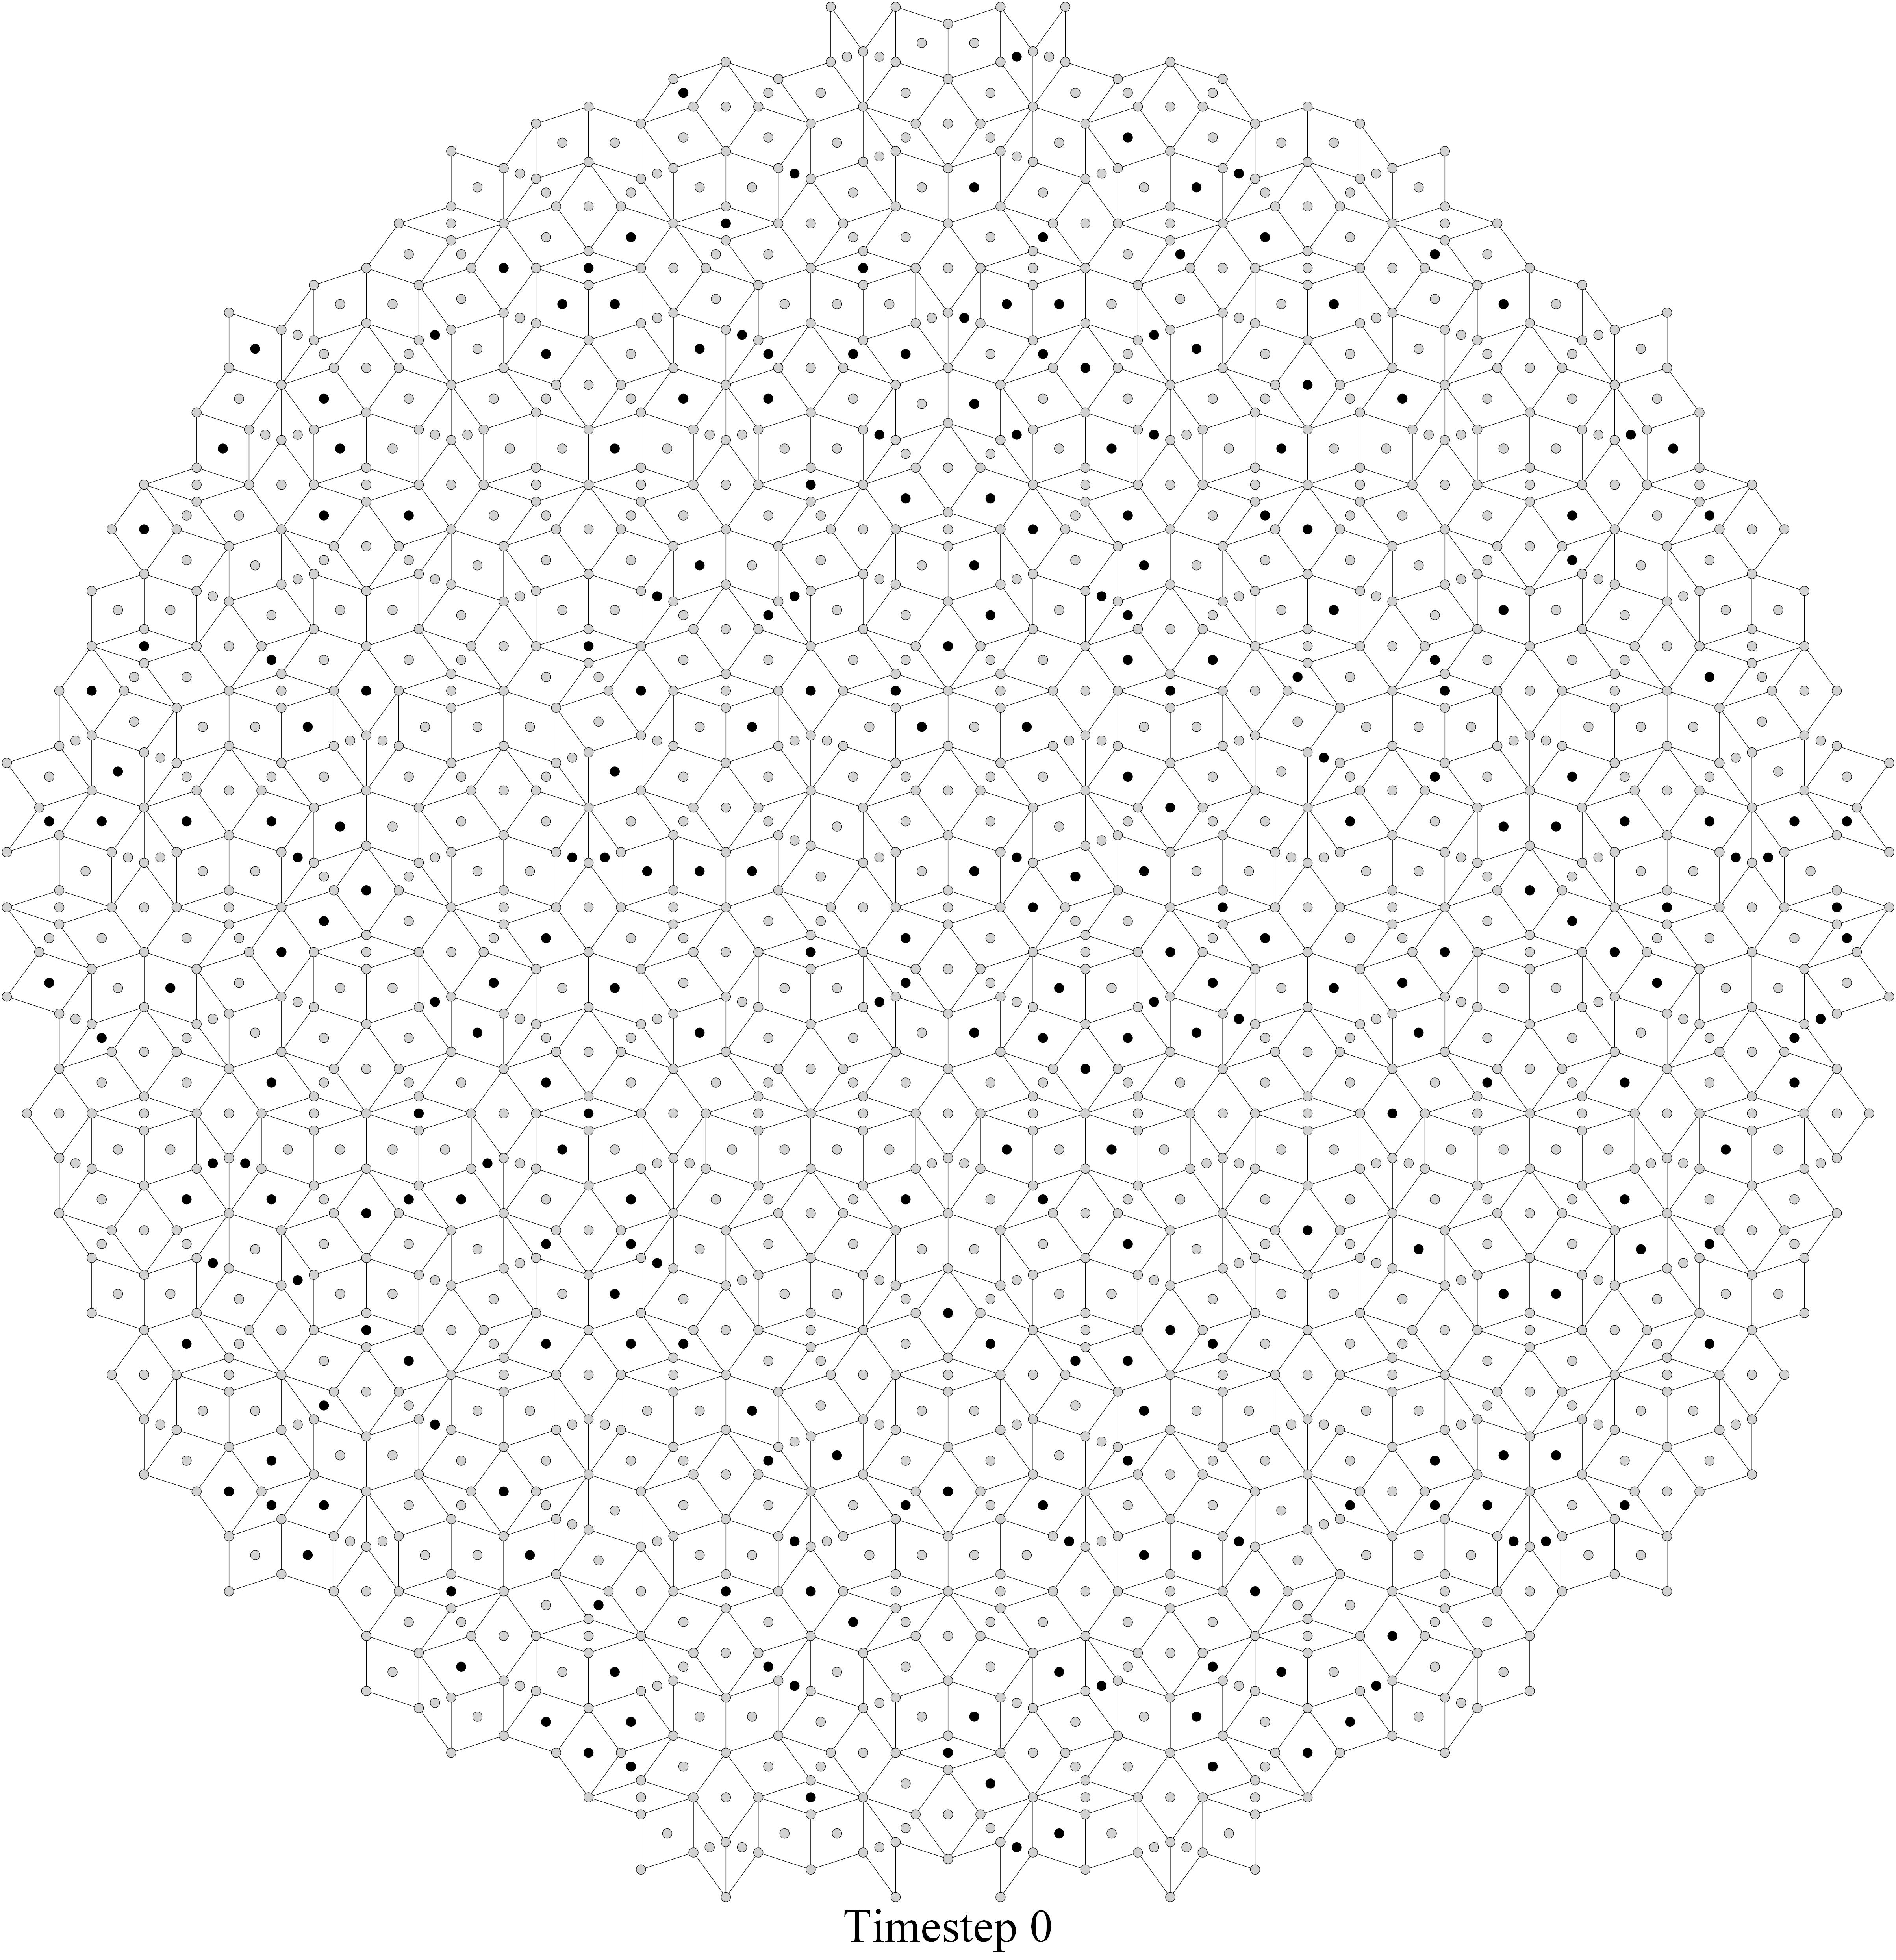
\includegraphics[width=0.2\columnwidth]{ch4_figs/crh_long/crh_long_0}}&")
  %print("\subcaptionbox{}{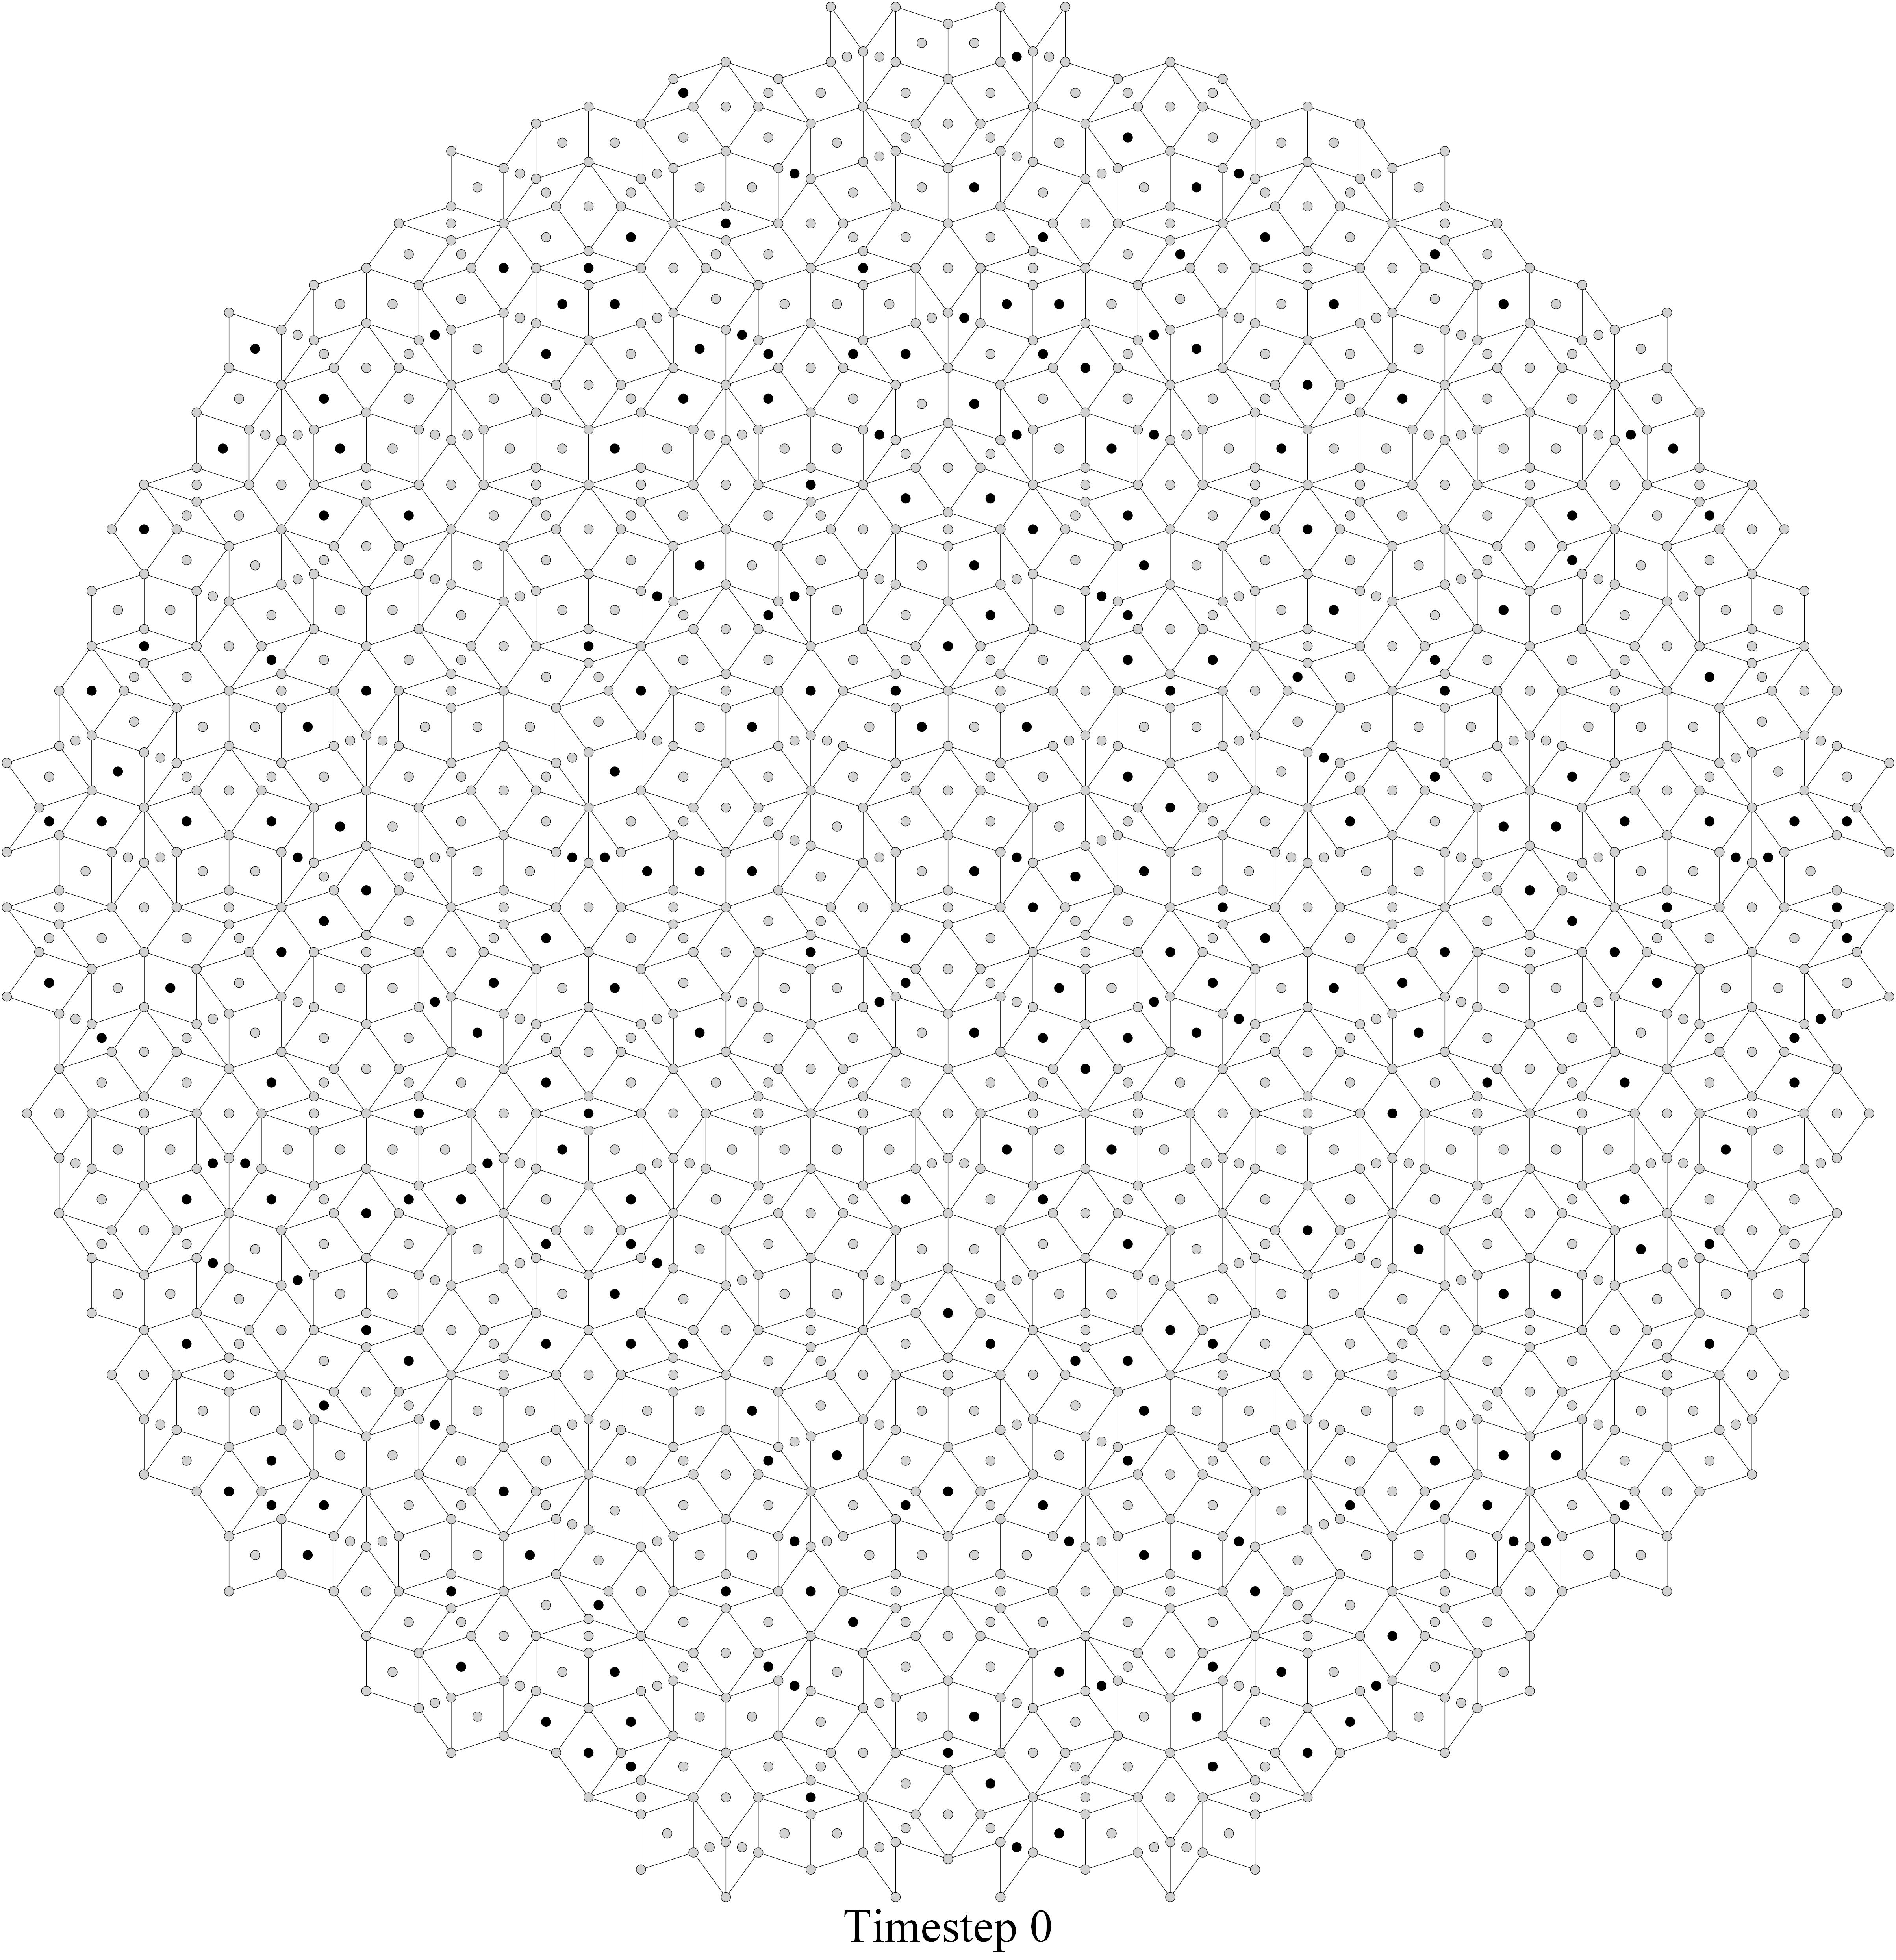
\includegraphics[width=0.2\columnwidth]{ch4_figs/crh_long/crh_long_0}}&")   
  %print("\subcaptionbox{}{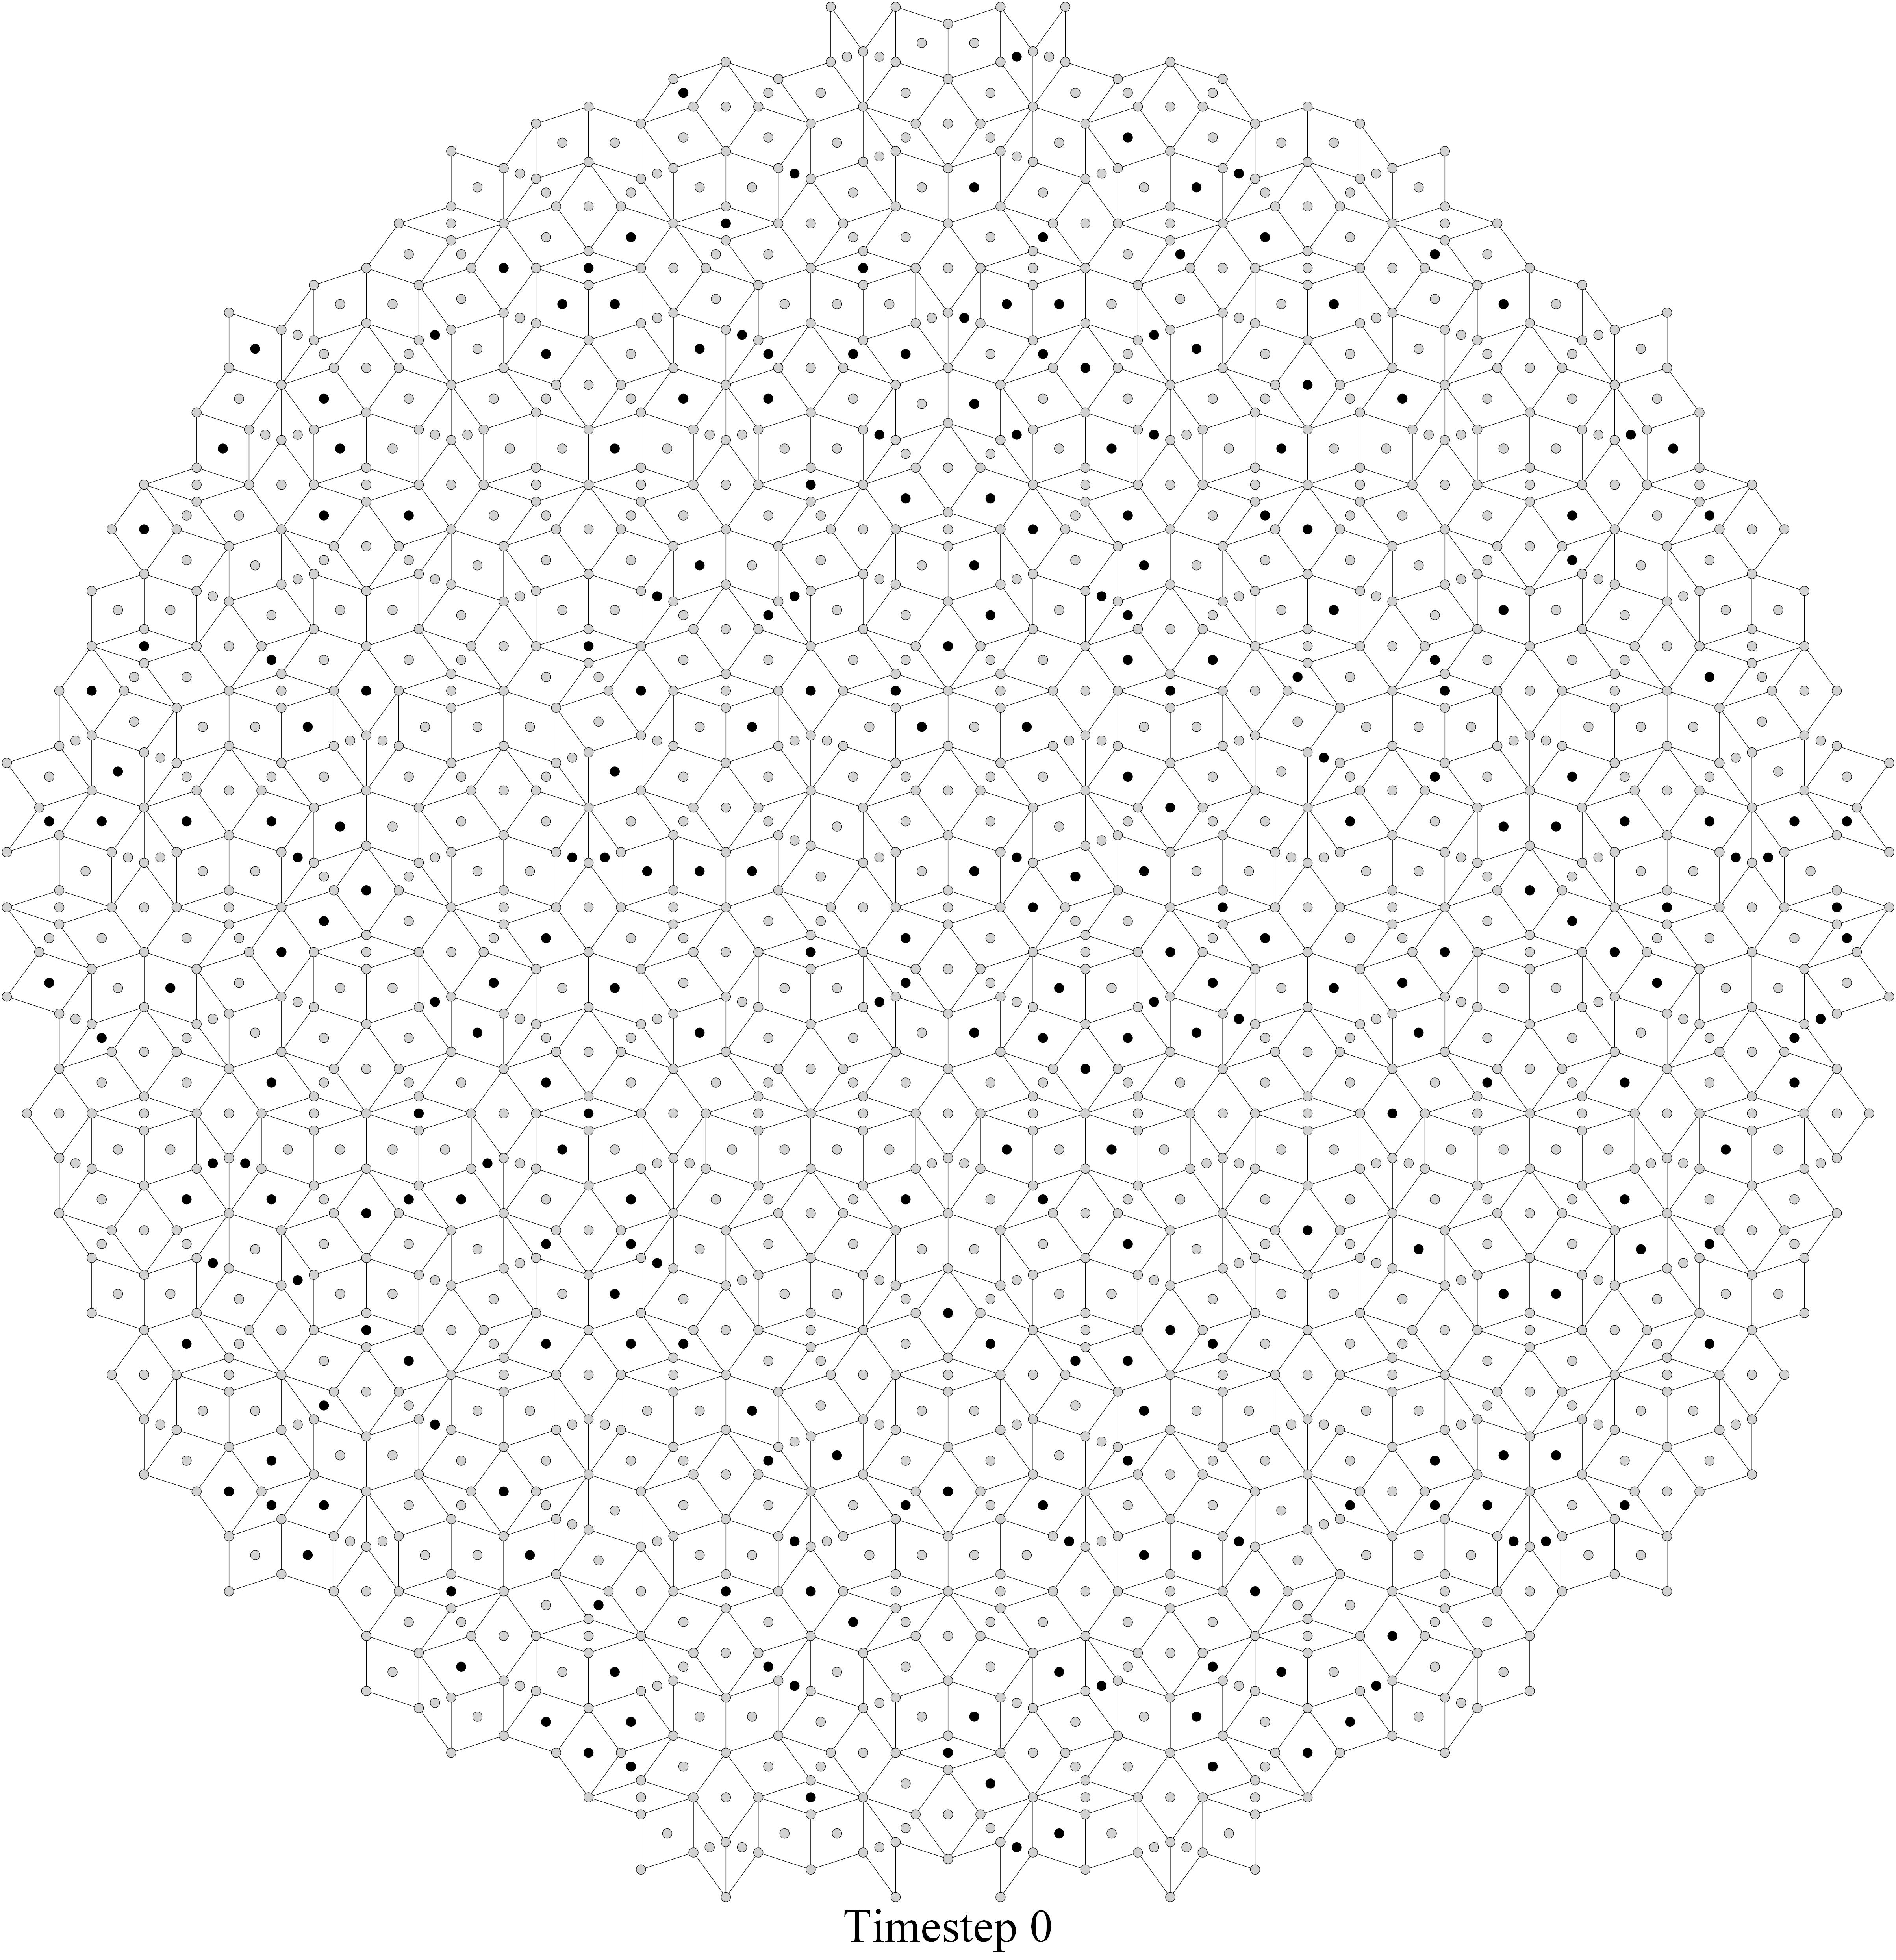
\includegraphics[width=0.2\columnwidth]{ch4_figs/crh_long/crh_long_0}}&")
  %print("\subcaptionbox{}{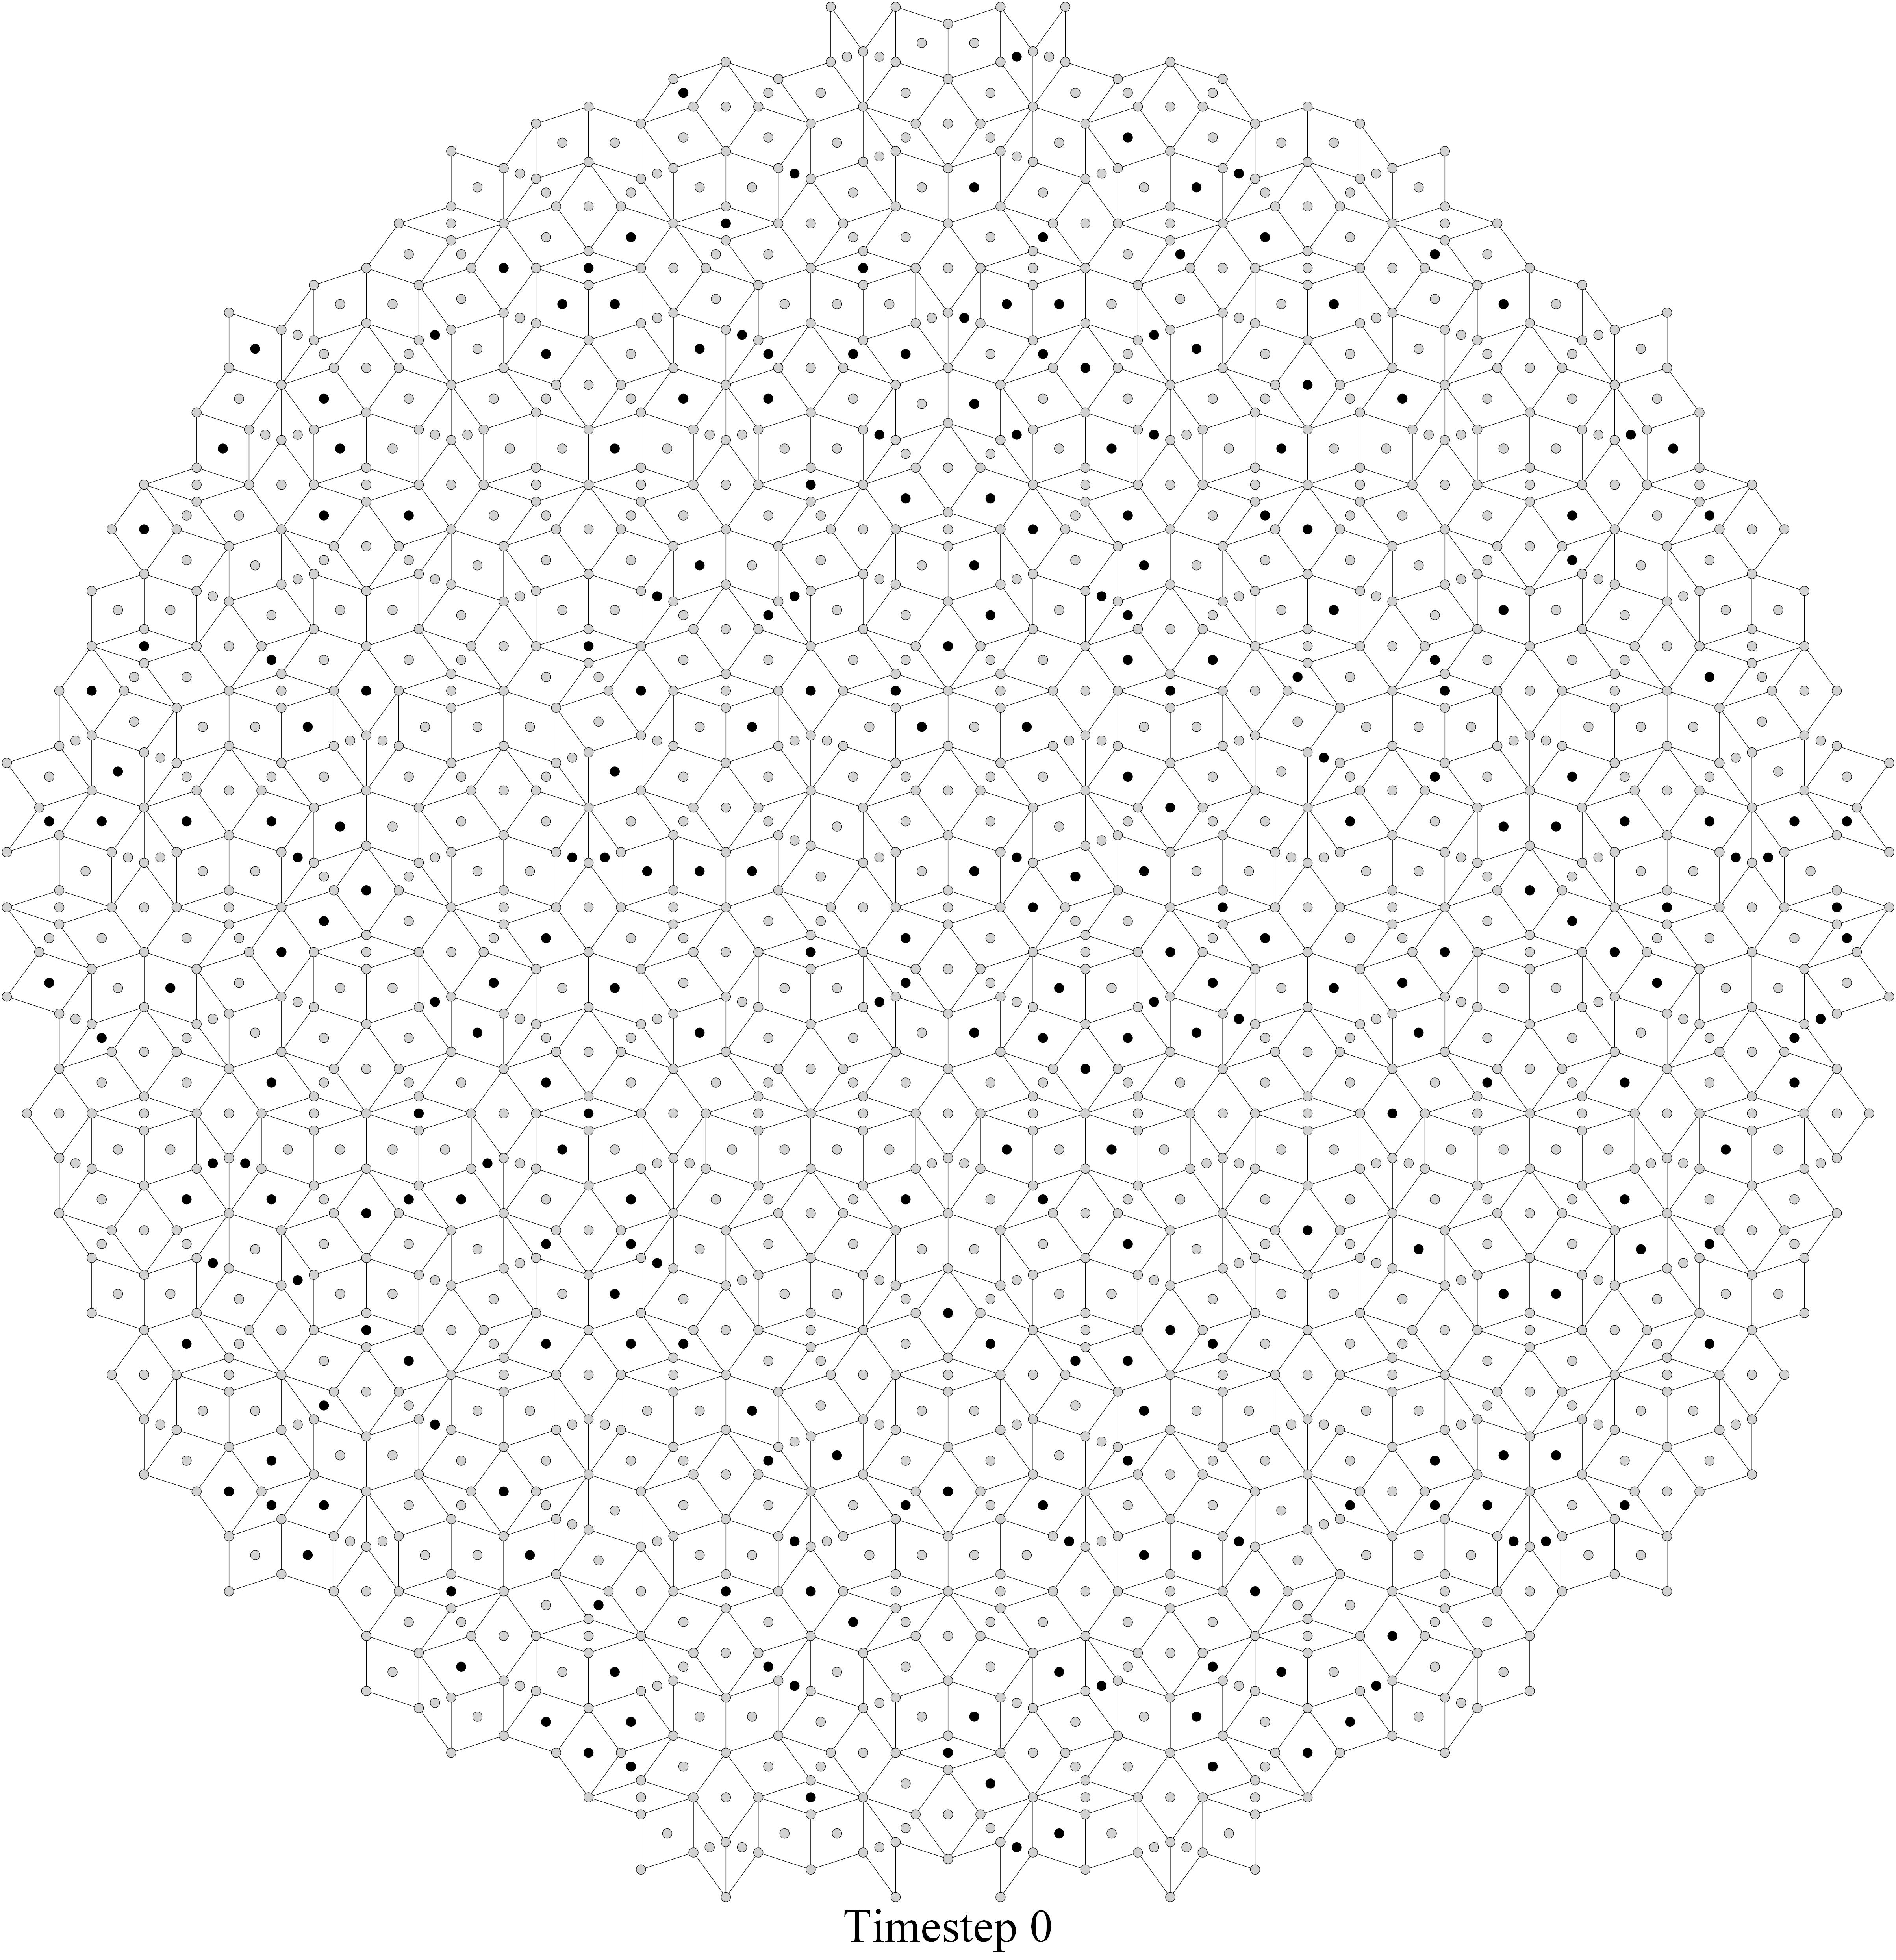
\includegraphics[width=0.2\columnwidth]{ch4_figs/crh_long/crh_long_0}}\\")
print("\\end{tabular}")
\end{python}
\fi
